\documentclass[11pt,a4paper]{article}
\usepackage[margin=2.1cm]{geometry}
\usepackage[T1]{fontenc}
\usepackage{lmodern}
\usepackage{microtype}
\usepackage{amsmath,amssymb,amsfonts,bm}
\usepackage{booktabs,array,multirow}
\usepackage{graphicx}
\usepackage{float}
\usepackage{caption}
\usepackage{xcolor}
\usepackage{enumitem}
\usepackage[most]{tcolorbox}
\usepackage[colorlinks=true,linkcolor=blue!50!black,urlcolor=blue!50!black,citecolor=blue!50!black]{hyperref}
\usepackage{algorithm}
\usepackage{algpseudocode}

\graphicspath{{../figures/}}
\captionsetup{font=small,labelfont=bf}
\setlength{\parskip}{4pt}
\setlength{\parindent}{0pt}
\renewcommand{\arraystretch}{1.12}

\newcommand{\PD}{\mathrm{PD}}
\newcommand{\LGD}{\mathrm{LGD}}
\newcommand{\EAD}{\mathrm{EAD}}
\newcommand{\ECL}{\mathrm{ECL}}
\newcommand{\VaR}{\mathrm{VaR}}
\newcommand{\ES}{\mathrm{ES}}
\newcommand{\logit}{\operatorname{logit}}
\newcommand{\Var}{\operatorname{Var}}
\newcommand{\E}{\mathbb{E}}
\newcommand{\1}{\mathbf{1}}

\tcbset{keybox/.style={colback=blue!4,colframe=blue!45!black,boxrule=0.6pt,arc=2pt,left=6pt,right=6pt,top=4pt,bottom=4pt,fonttitle=\bfseries}}
\newtcolorbox{keybox}[1][]{keybox,title=#1}
\newcounter{qn}
\newcommand{\Q}[1]{\refstepcounter{qn}\par\medskip\textbf{Q\theqn.\ #1}\par}
\newcommand{\A}{\textit{Answer.}\ }

\title{\textbf{Credit Risk Modelling \& Portfolio Stress Testing}\\[4pt]
\large PD, LGD, EAD, ECL, Monte Carlo VaR/ES and Stress Testing on 2.26 million LendingClub loans\\[2pt]
\normalsize Technical report: data, methodology, mathematics, statistical tests, results, and interview preparation}
\author{}
\date{}

\begin{document}
\sloppy
\maketitle
\thispagestyle{empty}

\begin{keybox}[Executive summary]
\begin{itemize}[leftmargin=*,itemsep=1pt]
\item \textbf{Data.} 2{,}260{,}701 accepted LendingClub loans (2007--2018Q4), snapshot March 2019. After cleaning, 2{,}257{,}919 loans; 1{,}762{,}677 have a complete 12-month outcome window (issued 2007--2017).
\item \textbf{Design flaw found and fixed.} The original ``terminal loans only'' design is survivorship-biased: the 2017 terminal subset has a 12-month default rate of \textbf{15.1\%} versus \textbf{5.8\%} for the whole 2017 cohort ($\chi^2$ $p\approx0$). The target was re-specified as a censoring-free \textbf{12-month PD} (Basel/IFRS~9 horizon).
\item \textbf{Out-of-time design.} Train 2007--2015 (884{,}691 loans), OOT test 2016 (434{,}407), OOT validation 2017 (443{,}579; \$6.585bn).
\item \textbf{PD.} LightGBM champion: \textbf{AUC 0.725, Gini 0.450, KS 0.325} on 2017; +0.023 AUC over the WOE logistic scorecard (DeLong $p<10^{-100}$).
\item \textbf{Calibration.} Raw PDs under-predict (4.80\% vs 5.80\%); Platt + grade recalibration (chosen on 2016 by LR test, $p=10^{-19}$) gives mean PD 5.90\%, ECE 0.24\,pp, Spiegelhalter $p=0.076$; no red grade in the Jeffreys backtest; score PSI 0.009.
\item \textbf{LGD / EAD.} LGD $=0.895$ (pooled; no model beats the mean OOT), downturn LGD $=0.936$; EAD fractional-logit model, OOT $R^2=0.29$.
\item \textbf{ECL.} 12-month ECL \textbf{\$321.5M} (4.88\%); realised \$326.1M (ratio 1.014). Lifetime ECL \$800.4M (12.15\%).
\item \textbf{Portfolio risk.} Loan-level one-factor Gaussian Monte Carlo (443{,}579 loans $\times$ 10{,}000 scenarios): EL \$320.5M, \textbf{99\% VaR \$723.7M, 99\% ES \$820.6M}, 99.9\% VaR \$939.8M. Combined adverse stress: 99\% VaR \$1{,}172.3M, ES \$1{,}343.1M. Reverse stress: PD odds $\times3.74$ make EL equal to base 99.9\% VaR.
\end{itemize}
\end{keybox}

\tableofcontents
\newpage

%=====================================================================
\section{Data}
%=====================================================================
\subsection{Source and cleaning}
\begin{itemize}[itemsep=1pt]
\item Source: Kaggle \texttt{wordsforthewise/lending-club}, file \texttt{accepted\_2007\_to\_2018Q4.csv.gz}: \textbf{2{,}260{,}701 rows, 151 columns}; issue dates June 2007 -- December 2018; the latest payment date in the file is \textbf{March 2019} (data snapshot).
\item Removed 33 rows with missing status/issue date and 2{,}749 ``Does not meet the credit policy'' loans (a different underwriting regime, 2007--2010): \textbf{2{,}257{,}919 loans} remain.
\item Loan status at snapshot: Fully Paid 1{,}076{,}751; Current 878{,}317; Charged Off 268{,}559; Late (31--120) 21{,}467; In Grace 8{,}436; Late (16--30) 4{,}349; Default 40.
\item Columns used: 67 application-time fields (model inputs) and 9 outcome fields (targets, LGD, EAD only).
\end{itemize}

\textbf{Leakage control.} Only information known at origination is a model input. Post-origination fields (payments, recoveries, \texttt{last\_fico}, \texttt{out\_prncp}, hardship and settlement flags, \texttt{last\_pymnt\_d}, \dots) are used \emph{only} to construct targets, LGD and EAD.

\begin{table}[H]\centering\small
\caption{Cohort summary. ``Terminal'' = Fully Paid / Charged Off / Default at the snapshot.}
\begin{tabular}{lrrrrr}
\toprule
Issue year & Loans & Funded (\$bn) & Terminal loans & Lifetime DR (terminal) & 12m DR (all loans) \\
\midrule
2007.0 & 251 & 0.002 & 251 & 17.93\% & 5.18\% \\
2008.0 & 1,562 & 0.013 & 1,562 & 15.81\% & 5.51\% \\
2009.0 & 4,716 & 0.046 & 4,716 & 12.60\% & 5.53\% \\
2010.0 & 11,536 & 0.117 & 11,536 & 12.89\% & 4.31\% \\
2011.0 & 21,721 & 0.257 & 21,721 & 15.18\% & 4.87\% \\
2012.0 & 53,367 & 0.718 & 53,367 & 16.20\% & 5.26\% \\
2013.0 & 134,814 & 1.983 & 134,804 & 15.60\% & 4.40\% \\
2014.0 & 235,629 & 3.504 & 223,103 & 18.45\% & 4.75\% \\
2015.0 & 421,095 & 6.418 & 375,546 & 20.19\% & 5.51\% \\
2016.0 & 434,407 & 6.401 & 293,105 & 23.29\% & 6.28\% \\
2017.0 & 443,579 & 6.585 & 169,321 & 23.13\% & 5.80\% \\
2018.0 & 495,242 & 7.936 & 56,318 & 15.76\% & -- \\
\bottomrule
\end{tabular}

\end{table}

\begin{figure}[H]\centering
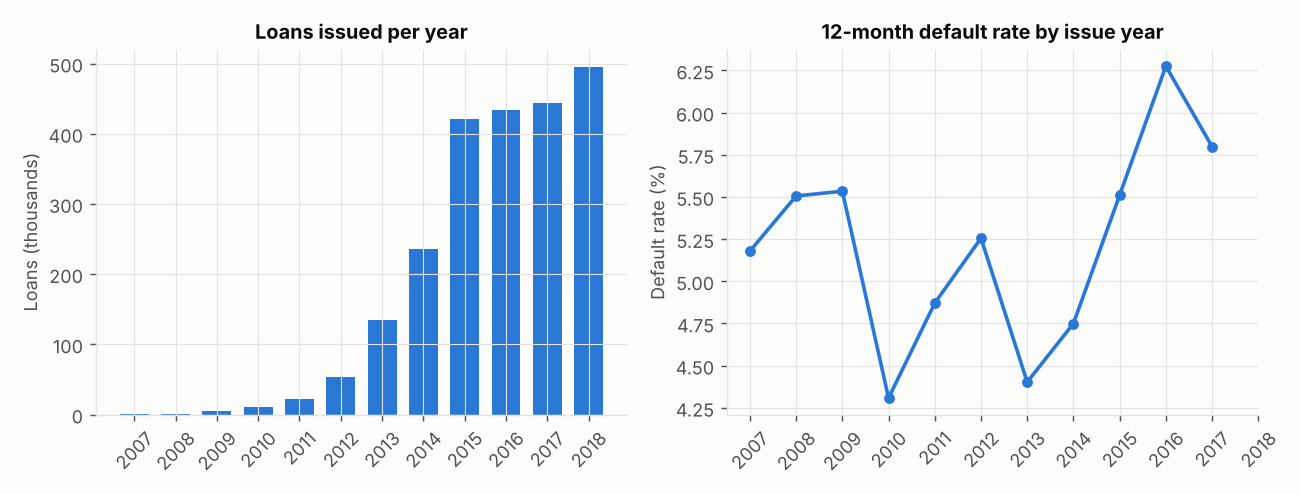
\includegraphics[width=\textwidth]{08_data_overview.png}
\caption{Loan volume and 12-month default rate by issue year (2018 has no complete 12-month window).}
\end{figure}

\subsection{Target definition: 12-month default}
Let $\mathcal{B}=\{\text{Charged Off},\ \text{Default},\ \text{Late (31--120 days)}\}$ be the set of default statuses. For loan $i$ with issue month $I_i$, last-payment month $LP_i$, recoveries $R_i$, principal and interest received $P_i,\ Int_i$ and instalment $A_i$, the month-on-book of the first missed instalment is
\begin{equation}
\tau_i=\operatorname{clip}\left(\begin{cases}
m(LP_i)-m(I_i)+1, & R_i=0 \text{ and } LP_i \text{ observed},\\[2pt]
\left\lceil \dfrac{P_i+Int_i}{A_i}\right\rceil+1, & \text{otherwise},
\end{cases}\ ,\ 1,\ \text{term}_i\right)
\end{equation}
The payment-count rule is used when recovery cash may have moved the last-payment date. On the 104{,}436 charge-offs without recoveries it agrees with the date rule on the 12-month flag in \textbf{98.0\%} of cases (mean bias $-0.11$ months). The target is
\begin{equation}
D_i=\1\{\text{status}_i\in\mathcal{B}\}\cdot\1\{\tau_i\le 12\},\qquad \text{defined for every loan with } I_i\le \text{Dec 2017}.
\end{equation}
Loans issued in December 2017 have their 12-month window close in December 2018; a miss at month 12 is $\ge$90 days past due by the March 2019 snapshot and is captured as Late (31--120) or Charged Off. Prepayment or survival beyond 12 months is $D_i=0$, so no loan is excluded because it is still open: \textbf{the target is free of survivorship bias}.

\subsection{Why the original design was replaced}
The original project used only \emph{terminal} loans with a lifetime target. For recent cohorts, only loans that had already ended are included, and those are disproportionately early charge-offs and early prepayments.

\begin{figure}[H]\centering
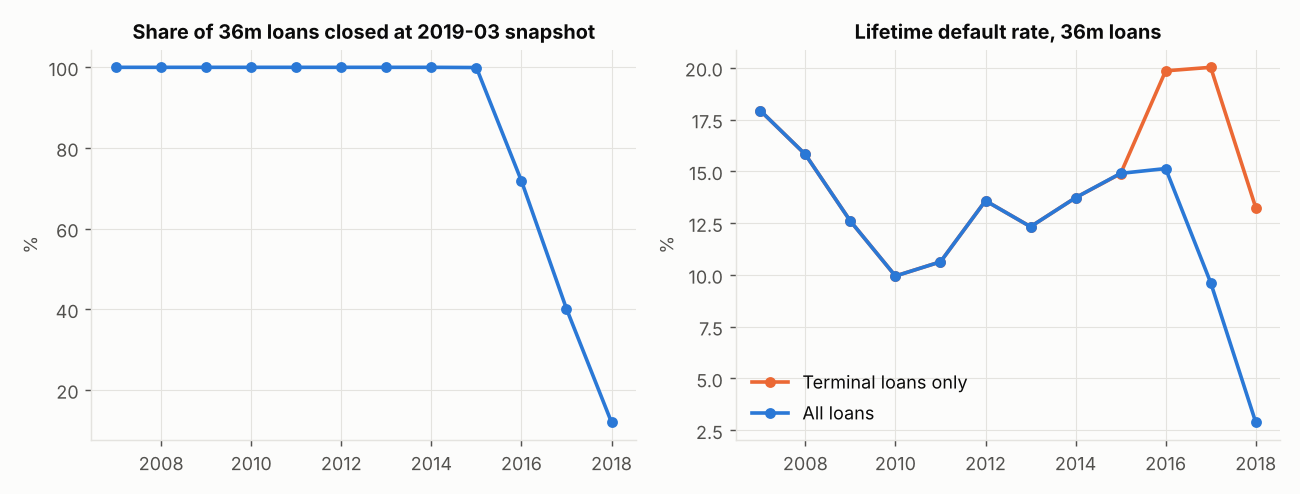
\includegraphics[width=\textwidth]{08_survivorship_bias.png}
\caption{36-month loans: once a cohort is fully matured (2007--2015) the terminal and full default rates coincide; for 2016--2017 the terminal subset strongly over-states default.}
\end{figure}

\begin{itemize}[itemsep=1pt]
\item 2017: 169{,}321 terminal loans = \textbf{38.2\%} of loans (36.8\% of dollars).
\item 12-month default rate: terminal subset \textbf{15.08\%} vs whole cohort \textbf{5.80\%}; $2\times2$ $\chi^2$ test terminal vs non-terminal: $p\approx 0$.
\item 76.9\% of the 2017 terminal loans are full early repayments; the remainder are early defaults.
\end{itemize}
Replicating the original design gives AUC 0.693 (LR) / 0.721 (LightGBM) and ECL \$454.2M on \$2.42bn, close to the original claim (AUC 0.700, ECL \$497.3M) -- but these figures describe a censored, selected sample, not the 2017 portfolio.

%=====================================================================
\section{Sample design (out-of-time)}
%=====================================================================
\begin{table}[H]\centering\small
\caption{Development, test and validation samples (12-month target).}
\begin{tabular}{llrrl}
\toprule
Sample & Issue years & Loans & 12m default rate & Role\\
\midrule
Development (train) & 2007--2015 & 884{,}691 & 5.09\% & model fitting\\
\quad tuning split A & 2007--2014 & 463{,}596 & -- & fit during hyper-parameter search\\
\quad tuning split B & 2015 & 421{,}095 & 5.51\% & early stopping / selection (time-based)\\
OOT test & 2016 & 434{,}407 & 6.28\% & champion choice, recalibration, stacking\\
OOT validation & 2017 & 443{,}579 & 5.80\% & final evaluation (scored once)\\
\bottomrule
\end{tabular}
\end{table}

\textbf{Protocol.} Every decision (variables, hyper-parameters, champion, recalibration method, stacking weights) uses data up to 2016 only. The 2017 cohort is never used for a choice.

\textbf{Training window test.} Bureau fields (e.g.\ \texttt{bc\_util}, \texttt{tot\_cur\_bal}) are 100\% missing before 2012. To check whether old vintages harm the model, LightGBM was trained on four windows ending 2014 and scored on 2015; paired DeLong tests show no significant difference, so the full window is kept.
\begin{table}[H]\centering\small
\caption{Training-window experiment (fixed LightGBM parameters).}
\begin{tabular}{lrrcr}
\toprule
Train window & $n$ train & AUC 2015 & 95\% CI & DeLong $p$ vs 2007--2014 \\
\midrule
2007-2014 & 463,596 & 0.7324 & [0.7293, 0.7356] & ref. \\
2010-2014 & 457,067 & 0.7327 & [0.7295, 0.7358] & 0.5202 \\
2012-2014 & 423,810 & 0.7331 & [0.7299, 0.7362] & 0.0966 \\
2013-2014 & 370,443 & 0.7328 & [0.7296, 0.7359] & 0.4124 \\
\bottomrule
\end{tabular}

\end{table}

%=====================================================================
\section{Features and feature selection}
%=====================================================================
\subsection{Candidate features}
68 candidates: 64 numeric and 4 categorical (\texttt{home\_ownership}, \texttt{verification\_status}, \texttt{purpose}, \texttt{addr\_state}). Engineered features:
\begin{align*}
\text{credit\_hist\_m}&=m(I_i)-m(\text{earliest credit line}), & \text{fico}&=\tfrac12(\text{fico\_low}+\text{fico\_high}),\\
\text{loan\_to\_inc}&=\frac{\text{loan amount}}{\text{annual income}}, & \text{inst\_to\_inc}&=\frac{12\cdot\text{instalment}}{\text{annual income}},\\
\text{revol\_to\_inc}&=\frac{\text{revolving balance}}{\text{annual income}}, & \text{log\_inc}&=\ln(1+\text{annual income}),
\end{align*}
plus \texttt{sub\_grade\_n} (A1$=1,\dots,$G5$=35$), employment length in years with a missing flag, joint-application and whole-loan flags; DTI outside $[0,100]$ is set missing.

\subsection{Weight of evidence and information value}
For a binned variable with bins $b=1,\dots,K$, $B_b$ defaults and $G_b$ non-defaults (with $+0.5$ smoothing),
\begin{equation}
\mathrm{WOE}_b=\ln\frac{B_b/B}{G_b/G},\qquad \mathrm{IV}=\sum_{b=1}^{K}\left(\frac{B_b}{B}-\frac{G_b}{G}\right)\mathrm{WOE}_b .
\end{equation}
Higher WOE means riskier, so every scorecard coefficient is expected to be positive.

\textbf{Monotone binning.} Numeric variables start from 20 quantile bins; adjacent bins are merged until (i) the default rate is monotone in the direction of the Spearman correlation between $x$ and $D$ and (ii) every bin holds $\ge5\%$ of the sample. Missing values form their own bin (WOE set to 0 if $<0.5\%$). Categorical levels below 0.5\% are pooled into ``OTHER''.

\begin{figure}[H]\centering
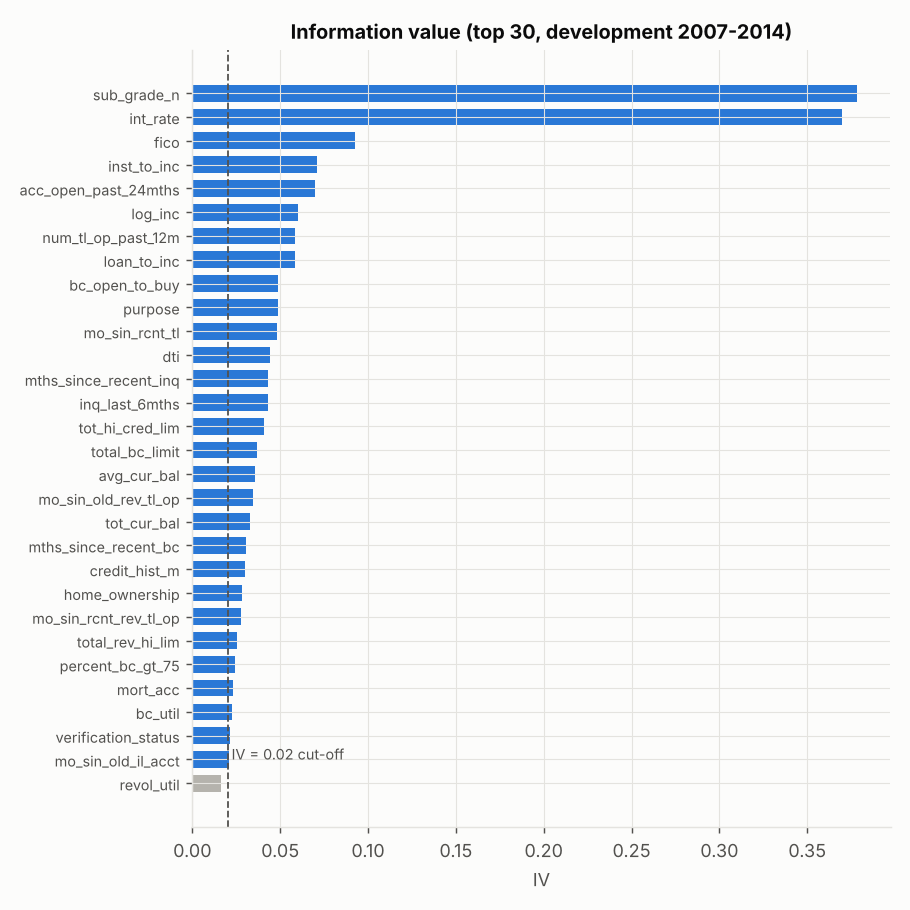
\includegraphics[width=0.72\textwidth]{08_information_value.png}
\caption{Information value of the top 30 candidates (development 2007--2014). 29 variables pass IV $\ge0.02$.}
\end{figure}

\subsection{Selection funnel for the logistic scorecard}
\begin{enumerate}[itemsep=1pt]
\item \textbf{IV filter}: IV $\ge0.02$ $\Rightarrow$ 29 variables.
\item \textbf{Correlation filter}: in IV order, drop a variable if $|r|>0.7$ with a stronger kept one $\Rightarrow$ 21 variables (e.g.\ \texttt{int\_rate} is dropped because it is collinear with \texttt{sub\_grade\_n}).
\item \textbf{Forward stepwise selection} on 2007--2014, holdout 2015. At each step every remaining variable is tried; the best is accepted only if \emph{all} gates pass:
\begin{itemize}[itemsep=0pt]
\item AUC gain on the 2015 holdout $\ge g_{\min}$ ($5\times10^{-4}$ for v1, $10^{-4}$ for v2);
\item Wald test $p<0.001$;
\item all coefficients positive (WOE sign consistency);
\item all VIF $<5$, where $\mathrm{VIF}_j=1/(1-R_j^2)$ and $R_j^2$ is from regressing WOE$_j$ on the other WOEs.
\end{itemize}
\end{enumerate}

\begin{table}[H]\centering\small
\caption{Forward stepwise path (scorecard v2). v1 stops after step 5.}
\begin{tabular}{rlrrr}
\toprule
Step & Variable added & Holdout AUC & AUC gain & Wald $p$ \\
\midrule
1 & sub\_grade\_n & 0.7042 & +0.2042 & $<10^{-299}$ \\
2 & acc\_open\_past\_24mths & 0.7130 & +0.0088 & $<10^{-140}$ \\
3 & home\_ownership & 0.7174 & +0.0044 & $<10^{-100}$ \\
4 & dti & 0.7184 & +0.0010 & $<10^{-50}$ \\
5 & mths\_since\_recent\_inq & 0.7196 & +0.0011 & $<10^{-28}$ \\
6 & mort\_acc & 0.7200 & +0.0004 & $<10^{-22}$ \\
7 & mo\_sin\_old\_il\_acct & 0.7202 & +0.0002 & $<10^{-45}$ \\
8 & verification\_status & 0.7205 & +0.0003 & 0.0006 \\
9 & mo\_sin\_old\_rev\_tl\_op & 0.7207 & +0.0001 & $<10^{-24}$ \\
10 & inq\_last\_6mths & 0.7208 & +0.0001 & $<10^{-24}$ \\
11 & mo\_sin\_rcnt\_tl & 0.7209 & +0.0001 & $<10^{-8}$ \\
12 & total\_rev\_hi\_lim & 0.7210 & +0.0001 & $<10^{-9}$ \\
\bottomrule
\end{tabular}

\end{table}

%=====================================================================
\section{Models}
%=====================================================================
\subsection{Logistic regression scorecard}
\begin{equation}
\logit\, P(D_i=1\mid\bm{x}_i)=\beta_0+\sum_{j\in S}\beta_j\,\mathrm{WOE}_j(x_{ij}),\qquad
\hat{\bm\beta}=\arg\max_{\bm\beta}\sum_i\big[D_i\ln p_i+(1-D_i)\ln(1-p_i)\big].
\end{equation}
Inference: Wald $z_j=\hat\beta_j/\widehat{SE}(\hat\beta_j)$; nested models are compared with the likelihood-ratio statistic $\Lambda=2(\ell_1-\ell_0)\sim\chi^2_{\Delta k}$; information criteria $\mathrm{AIC}=2k-2\ell$, $\mathrm{BIC}=k\ln n-2\ell$.

\begin{table}[H]\centering\small
\caption{Scorecard v1 (5 WOE variables), fitted on 2007--2015. LR test vs null $\chi^2=22{,}585$, pseudo-$R^2=0.063$.}
\begin{tabular}{lrrrrr}
\toprule
Term & $\hat\beta$ & SE & $z$ & $p$ & VIF \\
\midrule
const & -2.9268 & 0.0052 & -563.5 & $<10^{-299}$ & -- \\
sub\_grade\_n & 0.8930 & 0.0082 & 109.1 & $<10^{-299}$ & 1.10 \\
acc\_open\_past\_24mths & 0.5780 & 0.0161 & 35.9 & $<10^{-282}$ & 1.12 \\
home\_ownership & 0.9144 & 0.0272 & 33.7 & $<10^{-247}$ & 1.02 \\
dti & 0.4404 & 0.0200 & 22.0 & $<10^{-106}$ & 1.05 \\
mths\_since\_recent\_inq & 0.3340 & 0.0217 & 15.4 & $<10^{-52}$ & 1.11 \\
\bottomrule
\end{tabular}

\end{table}
\begin{table}[H]\centering\small
\caption{Scorecard v2 (12 WOE variables), fitted on 2007--2015.}
\begin{tabular}{lrrrrr}
\toprule
Term & $\hat\beta$ & SE & $z$ & $p$ & VIF \\
\midrule
const & -2.9273 & 0.0052 & -562.3 & $<10^{-299}$ & -- \\
sub\_grade\_n & 0.8372 & 0.0086 & 97.2 & $<10^{-299}$ & 1.29 \\
acc\_open\_past\_24mths & 0.5031 & 0.0183 & 27.5 & $<10^{-166}$ & 1.50 \\
home\_ownership & 0.6886 & 0.0308 & 22.3 & $<10^{-109}$ & 1.31 \\
dti & 0.4948 & 0.0205 & 24.1 & $<10^{-127}$ & 1.10 \\
mths\_since\_recent\_inq & 0.2078 & 0.0242 & 8.6 & $<10^{-17}$ & 1.33 \\
mort\_acc & 0.2031 & 0.0364 & 5.6 & $<10^{-7}$ & 1.44 \\
mo\_sin\_old\_il\_acct & 0.3825 & 0.0363 & 10.5 & $<10^{-25}$ & 1.15 \\
verification\_status & 0.2559 & 0.0247 & 10.4 & $<10^{-24}$ & 1.09 \\
mo\_sin\_old\_rev\_tl\_op & 0.3179 & 0.0272 & 11.7 & $<10^{-30}$ & 1.33 \\
inq\_last\_6mths & 0.2708 & 0.0250 & 10.8 & $<10^{-26}$ & 1.23 \\
mo\_sin\_rcnt\_tl & 0.1520 & 0.0245 & 6.2 & $<10^{-9}$ & 1.49 \\
total\_rev\_hi\_lim & 0.1891 & 0.0335 & 5.6 & $<10^{-7}$ & 1.28 \\
\bottomrule
\end{tabular}

\end{table}

\textbf{v2 vs v1.} Nested LR test $\chi^2=792.8$, df $=7$, $p=6.7\times10^{-167}$; AIC $333{,}498\to332{,}719$; BIC $333{,}568\to332{,}871$; DeLong on 2016: $\Delta$AUC $=+0.0011$, $z=3.40$, $p=0.0007$. v2 is statistically better but the economic gain is small.

\textbf{Scorecard points.} With PDO $=20$, 600 points at good:bad odds 50:1,
\begin{equation}
\text{Score}=\text{Offset}+\text{Factor}\cdot\ln(\text{odds}_{good}),\quad \text{Factor}=\frac{\text{PDO}}{\ln 2},\quad \text{Offset}=600-\text{Factor}\ln 50,
\end{equation}
and the points for attribute $b$ of variable $j$ are $-\left(\beta_j\mathrm{WOE}_{jb}+\beta_0/k\right)\text{Factor}+\text{Offset}/k$ (table \texttt{02\_scorecard\_points.csv}).

\subsection{Machine-learning challengers}
\textbf{Gradient boosting} builds an additive model $F_M(\bm x)=\sum_{m=1}^{M}\eta f_m(\bm x)$ of trees $f_m$ minimising the regularised log-loss
\begin{equation}
\mathcal{L}=\sum_i \ell\big(D_i,F(\bm x_i)\big)+\sum_m\Omega(f_m),\qquad \Omega(f)=\gamma T+\tfrac12\lambda\|\bm w\|^2,
\end{equation}
with $\ell$ the binary cross-entropy, $T$ leaves and leaf weights $\bm w$. Each tree fits the gradient $g_i=p_i-D_i$ and Hessian $h_i=p_i(1-p_i)$; the optimal leaf weight is $w_j^*=-\sum_{i\in j}g_i/(\sum_{i\in j}h_i+\lambda)$. LightGBM grows trees leaf-wise on histograms with native categorical splits; XGBoost grows depth-wise.
\textbf{Random forest}: average of 500 trees on 30\% bootstrap samples with random feature subsets.

\textbf{Tuning}: random search (LightGBM 20, XGBoost 12, RF 6 configurations), fitted on 2007--2014 with early stopping (100 rounds) on 2015; the selected number of rounds is scaled by $n_{2007\text{--}15}/n_{2007\text{--}14}=1.91$ for the final refit.
\begin{table}[H]\centering\small
\caption{Selected hyper-parameters. Best 2015 holdout AUC: LightGBM 0.7355, XGBoost 0.7344, RF 0.7246.}
\begin{tabular}{lp{12cm}}
\toprule
Model & Selected hyper-parameters (refit on 2007--2015) \\
\midrule
LightGBM & num\_leaves=63, min\_child\_samples=200, learning\_rate=0.03, feature\_fraction=0.5, bagging\_fraction=0.7, lambda\_l2=50.0, min\_split\_gain=0.0, n\_iter=1200 \\
XGBoost & max\_depth=8, min\_child\_weight=50.0, learning\_rate=0.03, subsample=0.9, colsample\_bytree=0.5, reg\_lambda=1.0, n\_iter=849 \\
Random Forest & min\_samples\_leaf=200, max\_features=0.2, n\_estimators=500, max\_samples=0.3 \\
\bottomrule
\end{tabular}

\end{table}

\begin{figure}[H]\centering
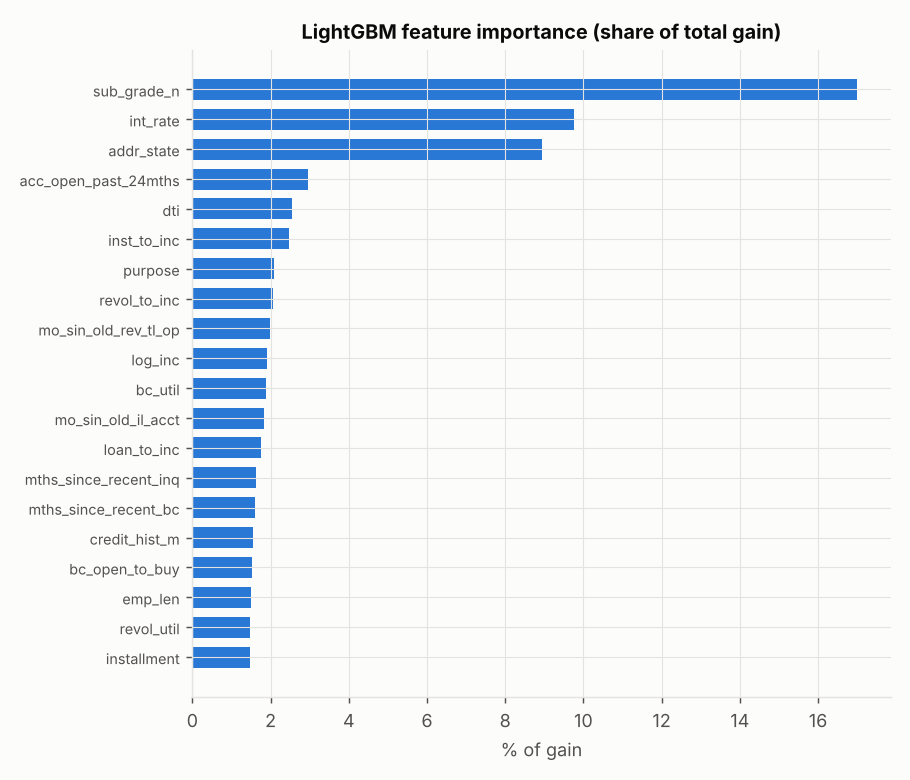
\includegraphics[width=0.66\textwidth]{08_lgb_importance.png}
\caption{LightGBM gain importance. Sub-grade, interest rate and state dominate; LendingClub's own grade already prices FICO and much of the bureau data.}
\end{figure}

\textbf{Stacking}: $\logit\,\hat p=\gamma_0+\gamma_1\logit p_{LR}+\gamma_2\logit p_{LGBM}+\gamma_3\logit p_{XGB}$ fitted on 2016; $\hat\gamma=(0.194, 0.136, 0.549, 0.295)$, all $p<10^{-13}$.

%=====================================================================
\section{Discrimination}
%=====================================================================
\subsection{Definitions}
For scores $s$ of defaulters ($m$ loans) and non-defaulters ($n$ loans),
\begin{align}
\mathrm{AUC}&=P(s_D>s_{ND})+\tfrac12P(s_D=s_{ND})=\frac{1}{mn}\sum_{i\in D}\sum_{j\in ND}\psi(s_i,s_j),\quad \psi=\1\{s_i>s_j\}+\tfrac12\1\{s_i=s_j\},\\
\mathrm{Gini}&=2\,\mathrm{AUC}-1,\qquad \mathrm{KS}=\max_t\big|F_{ND}(t)-F_{D}(t)\big|,\\
\text{Brier}&=\frac1N\sum_i(\hat p_i-D_i)^2,\qquad \text{Log-loss}=-\frac1N\sum_i\big[D_i\ln\hat p_i+(1-D_i)\ln(1-\hat p_i)\big].
\end{align}

\textbf{DeLong test.} With structural components $V_{10}(s_i)=\frac1n\sum_j\psi(s_i,s_j)$ and $V_{01}(s_j)=\frac1m\sum_i\psi(s_i,s_j)$, the covariance of AUC estimates for models $r,s$ is
\begin{equation}
\widehat{\mathrm{Cov}}(\widehat{A}_r,\widehat{A}_s)=\frac{S_{10}^{rs}}{m}+\frac{S_{01}^{rs}}{n},\qquad
z=\frac{\widehat A_1-\widehat A_2}{\sqrt{\Var(\widehat A_1)+\Var(\widehat A_2)-2\mathrm{Cov}(\widehat A_1,\widehat A_2)}}\sim N(0,1),
\end{equation}
computed with the $O(N\log N)$ algorithm of Sun \& Xu (2014). With 15 pairwise tests, $p$-values are Holm-adjusted: $p_{(k)}^{adj}=\max_{j\le k}\min\{1,(M-j+1)p_{(j)}\}$.

\subsection{Results}
\begin{table}[H]\centering\small
\caption{Out-of-time discrimination of the raw models (2016 test, 2017 validation).}
\begin{tabular}{llrcrrrr}
\toprule
Sample & Model & AUC & 95\% DeLong CI & Gini & KS & Brier & Log-loss \\
\midrule
test 2016 & LogReg\_WOE & 0.7108 & [0.7077, 0.7138] & 0.4216 & 0.3058 & 0.0569 & 0.2190 \\
test 2016 & LightGBM & 0.7326 & [0.7297, 0.7356] & 0.4652 & 0.3396 & 0.0561 & 0.2146 \\
test 2016 & XGBoost & 0.7313 & [0.7284, 0.7343] & 0.4626 & 0.3373 & 0.0562 & 0.2151 \\
test 2016 & RandomForest & 0.7209 & [0.7179, 0.7239] & 0.4418 & 0.3212 & 0.0566 & 0.2170 \\
valid 2017 & LogReg\_WOE & 0.7021 & [0.6989, 0.7053] & 0.4042 & 0.2915 & 0.0531 & 0.2080 \\
valid 2017 & LightGBM & 0.7252 & [0.7221, 0.7282] & 0.4503 & 0.3253 & 0.0524 & 0.2041 \\
valid 2017 & XGBoost & 0.7238 & [0.7208, 0.7269] & 0.4477 & 0.3229 & 0.0525 & 0.2045 \\
valid 2017 & RandomForest & 0.7144 & [0.7112, 0.7175] & 0.4287 & 0.3091 & 0.0527 & 0.2056 \\
\bottomrule
\end{tabular}

\end{table}

\begin{table}[H]\centering\small
\caption{2017 validation including scorecard v2 and stacking.}
\begin{tabular}{lrcrr}
\toprule
Model (2017) & AUC & 95\% CI & Gini & KS \\
\midrule
LogReg\_WOE & 0.7021 & [0.6989, 0.7053] & 0.4042 & 0.2915 \\
LightGBM & 0.7252 & [0.7221, 0.7282] & 0.4503 & 0.3253 \\
XGBoost & 0.7238 & [0.7208, 0.7269] & 0.4477 & 0.3229 \\
RandomForest & 0.7144 & [0.7112, 0.7175] & 0.4287 & 0.3091 \\
LogReg\_WOE\_v2 & 0.7035 & [0.7004, 0.7067] & 0.4071 & 0.2956 \\
Stacked & 0.7260 & [0.7230, 0.7291] & 0.4521 & 0.3266 \\
\bottomrule
\end{tabular}

\end{table}

\begin{table}[H]\centering\small
\caption{Paired DeLong tests on 2017 with Holm correction ($\Delta$AUC = A $-$ B).}
\begin{tabular}{lrrrr}
\toprule
Comparison (A vs B) & $\Delta$AUC & $z$ & $p$ & $p$ (Holm) \\
\midrule
LogReg\_WOE vs LightGBM & -0.0231 & -24.03 & $<10^{-126}$ & $<10^{-125}$ \\
LogReg\_WOE vs XGBoost & -0.0217 & -22.44 & $<10^{-110}$ & $<10^{-109}$ \\
LogReg\_WOE vs RandomForest & -0.0123 & -20.47 & $<10^{-92}$ & $<10^{-91}$ \\
LogReg\_WOE vs LogReg\_WOE\_v2 & -0.0014 & -4.14 & $<10^{-4}$ & $<10^{-4}$ \\
LogReg\_WOE vs Stacked & -0.0239 & -27.90 & $<10^{-170}$ & $<10^{-169}$ \\
LightGBM vs XGBoost & +0.0013 & 3.65 & 0.0003 & 0.0003 \\
LightGBM vs RandomForest & +0.0108 & 14.69 & $<10^{-48}$ & $<10^{-47}$ \\
LightGBM vs LogReg\_WOE\_v2 & +0.0216 & 23.34 & $<10^{-119}$ & $<10^{-118}$ \\
LightGBM vs Stacked & -0.0009 & -5.23 & $<10^{-6}$ & $<10^{-6}$ \\
XGBoost vs RandomForest & +0.0095 & 12.71 & $<10^{-36}$ & $<10^{-35}$ \\
XGBoost vs LogReg\_WOE\_v2 & +0.0203 & 21.77 & $<10^{-104}$ & $<10^{-103}$ \\
XGBoost vs Stacked & -0.0022 & -8.54 & $<10^{-16}$ & $<10^{-16}$ \\
RandomForest vs LogReg\_WOE\_v2 & +0.0108 & 19.52 & $<10^{-84}$ & $<10^{-83}$ \\
RandomForest vs Stacked & -0.0117 & -18.16 & $<10^{-72}$ & $<10^{-72}$ \\
LogReg\_WOE\_v2 vs Stacked & -0.0225 & -27.62 & $<10^{-167}$ & $<10^{-165}$ \\
\bottomrule
\end{tabular}

\end{table}

\begin{figure}[H]\centering
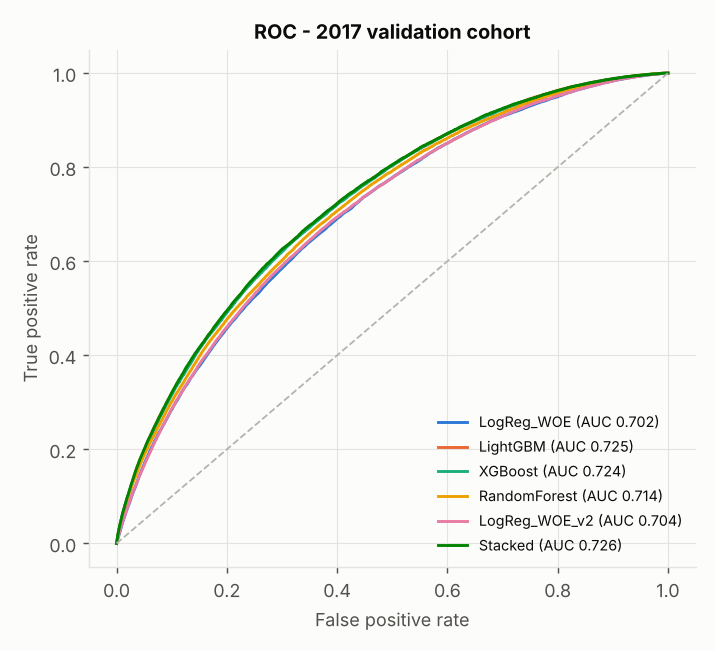
\includegraphics[width=0.55\textwidth]{03_roc_2017.png}
\caption{ROC curves on the 2017 validation cohort.}
\end{figure}

\begin{figure}[H]\centering
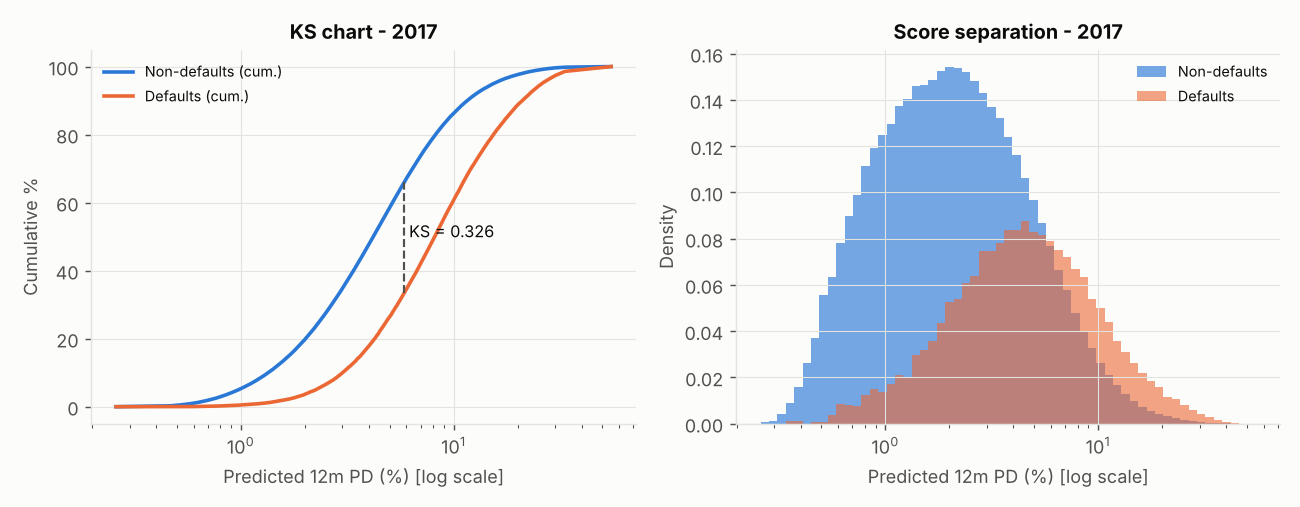
\includegraphics[width=\textwidth]{08_ks_score_distribution.png}
\caption{KS chart and score separation of the final PD, 2017.}
\end{figure}

\textbf{Conclusion.} The champion was chosen on 2016 AUC (LightGBM 0.7326). On 2017 it beats the scorecard by $+0.023$ AUC (LR v1) and $+0.022$ (LR v2), XGBoost by $+0.0013$ ($p_{Holm}=0.0003$) and RF by $+0.011$, all significant. Stacking adds $+0.0009$ AUC: significant but immaterial, so the single LightGBM is retained for simplicity.

%=====================================================================
\section{Calibration and recalibration}
%=====================================================================
\subsection{Calibration statistics}
\begin{itemize}[itemsep=2pt]
\item \textbf{Calibration intercept/slope} (logistic recalibration): $\logit P(D=1)=a+b\,\logit\hat p$. Calibration-in-the-large (CITL) is $a$ with $b$ fixed to 1 (offset). Ideal: $a=0$, $b=1$; Wald tests $H_0:a=0$ and $H_0:b=1$.
\item \textbf{Hosmer--Lemeshow} over $G=10$ PD deciles: $\displaystyle \mathrm{HL}=\sum_{g=1}^{G}\frac{(O_g-E_g)^2}{N_g\bar p_g(1-\bar p_g)}\sim\chi^2_{G-2}$.
\item \textbf{Spiegelhalter} $\displaystyle Z=\frac{\sum_i(D_i-\hat p_i)(1-2\hat p_i)}{\sqrt{\sum_i(1-2\hat p_i)^2\hat p_i(1-\hat p_i)}}\sim N(0,1)$.
\item \textbf{Expected calibration error} over 20 equal-frequency bins: $\mathrm{ECE}=\sum_b\frac{N_b}{N}\left|\bar D_b-\bar p_b\right|$.
\end{itemize}
With $N=443{,}579$, HL has very high power and rejects deviations of a few basis points, so it is always reported alongside effect sizes (ECE, CITL).

\subsection{Recalibration methods (fitted on 2016, applied to 2017)}
\begin{align}
\text{Intercept shift:}&\quad \hat p'=\Lambda(\logit\hat p+a),\ \ a \text{ solves } \tfrac1N\textstyle\sum_i\Lambda(\logit\hat p_i+a)=\bar D_{2016},\\
\text{Platt:}&\quad \hat p'=\Lambda(a+b\,\logit\hat p),\\
\text{Isotonic:}&\quad \hat p'=\hat m(\hat p),\ \hat m=\arg\min_{m\ \uparrow}\textstyle\sum_i(D_i-m(\hat p_i))^2\ \text{(pool-adjacent-violators)},\\
\text{Platt + grade:}&\quad \hat p'=\Lambda\big(a+b\,\logit\hat p+\textstyle\sum_{g\neq A}\gamma_g\1\{\text{grade}=g\}\big),
\end{align}
with $\Lambda(x)=1/(1+e^{-x})$.

\textbf{Pre-specified decision rule (2016 evidence only).}
\begin{enumerate}[itemsep=1pt]
\item 2016 slope of the champion $=0.924$, 95\% CI $[0.910,0.938]$, $p(b=1)=3.2\times10^{-26}$ $\Rightarrow$ Platt instead of intercept shift.
\item Residual grade effect after Platt: LR test Platt+grade vs Platt, $\chi^2=101.4$, df $=6$, $p=1.3\times10^{-19}$ $\Rightarrow$ adopt Platt + grade (grades D and E were under-predicted in 2016).
\end{enumerate}

\begin{table}[H]\centering
\caption{2017 calibration of every model and method (raw models under-predict: mean PD $\approx4.8\%$ vs DR 5.80\%).}
\resizebox{\textwidth}{!}{\begin{tabular}{llrrrrrrrrr}
\toprule
Model & Method & PD\% & CITL & $p$ & Slope & $p$(=1) & HL $\chi^2_8$ & Spieg. $p$ & ECE pp & Brier \\
\midrule
LogReg\_WOE & raw & 4.76 & +0.215 & $<10^{-237}$ & 1.028 & 0.0039 & 1120.0 & $<10^{-232}$ & 1.04 & 0.0531 \\
LogReg\_WOE & intercept\_shift & 5.91 & -0.021 & 0.0012 & 1.028 & 0.0039 & 36.4 & 0.0003 & 0.20 & 0.0529 \\
LogReg\_WOE & platt & 5.89 & -0.017 & 0.0079 & 0.977 & 0.0151 & 29.8 & 0.0147 & 0.17 & 0.0529 \\
LogReg\_WOE & isotonic & 5.88 & -0.016 & 0.0136 & 0.975 & 0.0071 & 23.4 & 0.0348 & 0.18 & 0.0529 \\
LightGBM & raw & 4.80 & +0.210 & $<10^{-220}$ & 0.894 & $<10^{-47}$ & 1279.3 & $<10^{-259}$ & 1.00 & 0.0524 \\
LightGBM & intercept\_shift & 5.88 & -0.016 & 0.0136 & 0.894 & $<10^{-47}$ & 215.3 & 0.3639 & 0.40 & 0.0524 \\
LightGBM & platt & 5.91 & -0.022 & 0.0011 & 0.968 & $<10^{-4}$ & 69.4 & 0.0486 & 0.20 & 0.0523 \\
LightGBM & isotonic & 5.91 & -0.021 & 0.0013 & 0.958 & $<10^{-6}$ & 41.5 & 0.0221 & 0.23 & 0.0523 \\
XGBoost & raw & 4.70 & +0.233 & $<10^{-271}$ & 0.917 & $<10^{-26}$ & 1397.1 & $<10^{-299}$ & 1.10 & 0.0525 \\
XGBoost & intercept\_shift & 5.86 & -0.012 & 0.0635 & 0.917 & $<10^{-26}$ & 116.6 & 0.6877 & 0.31 & 0.0524 \\
XGBoost & platt & 5.89 & -0.018 & 0.0074 & 0.983 & 0.0380 & 30.0 & 0.0492 & 0.17 & 0.0523 \\
XGBoost & isotonic & 5.89 & -0.018 & 0.0056 & 0.973 & 0.0010 & 25.1 & 0.0250 & 0.16 & 0.0523 \\
RandomForest & raw & 4.86 & +0.192 & $<10^{-189}$ & 1.075 & $<10^{-14}$ & 933.0 & $<10^{-178}$ & 0.95 & 0.0527 \\
RandomForest & intercept\_shift & 6.04 & -0.045 & $<10^{-11}$ & 1.075 & $<10^{-14}$ & 103.3 & $<10^{-14}$ & 0.33 & 0.0526 \\
RandomForest & platt & 6.02 & -0.041 & $<10^{-9}$ & 0.981 & 0.0250 & 57.7 & $<10^{-8}$ & 0.23 & 0.0526 \\
RandomForest & isotonic & 6.02 & -0.041 & $<10^{-9}$ & 0.975 & 0.0044 & 54.9 & $<10^{-8}$ & 0.23 & 0.0526 \\
LogReg\_WOE\_v2 & raw & 4.74 & +0.220 & $<10^{-247}$ & 1.012 & 0.1954 & 1156.2 & $<10^{-244}$ & 1.06 & 0.0530 \\
LogReg\_WOE\_v2 & intercept\_shift & 5.89 & -0.017 & 0.0080 & 1.012 & 0.1954 & 26.9 & 0.0051 & 0.15 & 0.0529 \\
LogReg\_WOE\_v2 & platt & 5.88 & -0.015 & 0.0231 & 0.980 & 0.0343 & 26.4 & 0.0410 & 0.15 & 0.0529 \\
LogReg\_WOE\_v2 & isotonic & 5.87 & -0.014 & 0.0302 & 0.976 & 0.0085 & 27.1 & 0.0722 & 0.19 & 0.0529 \\
Stacked & raw & 5.88 & -0.016 & 0.0175 & 0.977 & 0.0034 & 34.1 & 0.1261 & 0.17 & 0.0523 \\
\bottomrule
\end{tabular}
}
\end{table}

\begin{table}[H]\centering
\caption{Final calibration on 2017 with 95\% confidence intervals.}
\resizebox{\textwidth}{!}{\begin{tabular}{lrccrcr}
\toprule
Model (2017, DR 5.80\%) & Mean PD & CITL [95\% CI] & Slope [95\% CI] & HL $\chi^2_8$ & Spiegelhalter $z$ ($p$) & ECE pp \\
\midrule
LightGBM + Platt & 5.91\% & -0.0215 [-0.034, -0.009] & 0.9677 [0.952, 0.983] & 69.4 & -1.97 (0.049) & 0.20 \\
LightGBM + Platt + grade (final) & 5.90\% & -0.0196 [-0.033, -0.007] & 0.9692 [0.954, 0.985] & 81.8 & -1.77 (0.076) & 0.24 \\
LogReg v2 + Platt & 5.88\% & -0.0148 [-0.028, -0.002] & 0.9804 [0.962, 0.999] & 26.4 & -2.04 (0.041) & 0.15 \\
\bottomrule
\end{tabular}
}
\end{table}

\begin{figure}[H]\centering
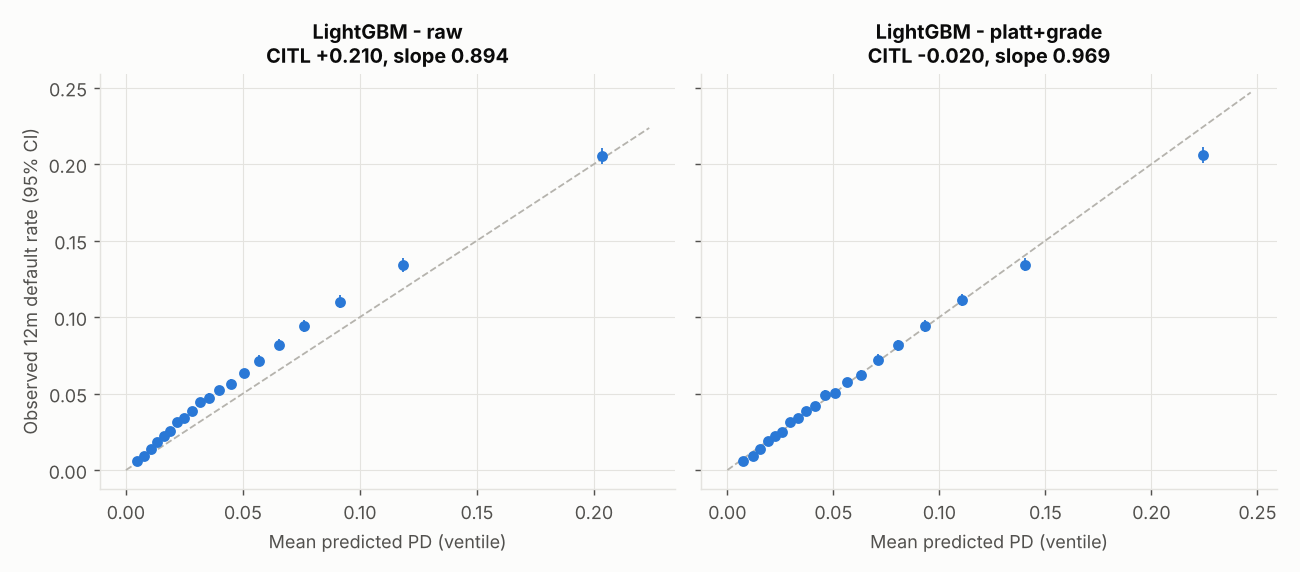
\includegraphics[width=\textwidth]{03_calibration_2017.png}
\caption{Reliability diagram (20 ventiles, 95\% binomial CI): raw LightGBM vs Platt + grade.}
\end{figure}

\textbf{Interpretation.} Recalibration moves mean PD from 4.80\% to 5.90\% (observed 5.80\%), CITL from $+0.210$ to $-0.020$ (slightly conservative), ECE from 1.00\,pp to 0.24\,pp; Spiegelhalter $p=0.076$ (no overall miscalibration at 5\%). The residual slope $0.969<1$ means the extreme PDs are slightly too spread; the HL statistic (81.8) is driven by the top decile, where PD over-states the default rate (conservative).

%=====================================================================
\section{Backtesting}
%=====================================================================
For a bucket with $N$ loans, $D$ defaults and mean PD $\bar p$:
\begin{itemize}[itemsep=2pt]
\item \textbf{Exact binomial test} $H_0: \text{DR}=\bar p$, $D\sim\mathrm{Bin}(N,\bar p)$, two-sided.
\item \textbf{Jeffreys test} (ECB TRIM): posterior $\text{DR}\mid D\sim\mathrm{Beta}(D+\tfrac12,\,N-D+\tfrac12)$, $p=F_{\mathrm{Beta}}(\bar p)=P(\text{DR}\le\bar p\mid D)$. A small $p$ means PD is too low.
\item \textbf{Traffic light}: red if $p<0.01$, amber if $p<0.05$, ``conservative'' if $p>0.99$, otherwise green.
\end{itemize}

\begin{table}[H]\centering\small
\caption{Backtest by grade, 2017 (final PD).}
\begin{tabular}{lrrrrrrl}
\toprule
Grade & $N$ & $D$ & Mean PD & ODR & Binomial $p$ & Jeffreys $p$ & Light \\
\midrule
A & 78,796 & 1,202 & 1.59\% & 1.53\% & 0.1756 & 0.9153 & green \\
B & 133,127 & 4,670 & 3.50\% & 3.51\% & 0.9287 & 0.4647 & green \\
C & 145,144 & 8,978 & 6.20\% & 6.19\% & 0.8319 & 0.5855 & green \\
D & 56,646 & 5,816 & 10.27\% & 10.27\% & 0.9945 & 0.4975 & green \\
E & 20,167 & 2,971 & 15.89\% & 14.73\% & $<10^{-5}$ & 1.0000 & conservative \\
F & 6,242 & 1,239 & 22.55\% & 19.85\% & $<10^{-6}$ & 1.0000 & conservative \\
G & 3,457 & 844 & 24.17\% & 24.41\% & 0.7356 & 0.3664 & green \\
\bottomrule
\end{tabular}

\end{table}
\begin{table}[H]\centering\small
\caption{Backtest by PD decile, 2017.}
\begin{tabular}{lrrrrrrl}
\toprule
Pd Decile & $N$ & $D$ & Mean PD & ODR & Binomial $p$ & Jeffreys $p$ & Light \\
\midrule
1 & 44,358 & 330 & 0.97\% & 0.74\% & $<10^{-6}$ & 1.0000 & conservative \\
2 & 44,358 & 723 & 1.73\% & 1.63\% & 0.0943 & 0.9553 & green \\
3 & 44,358 & 1,052 & 2.42\% & 2.37\% & 0.5466 & 0.7305 & green \\
4 & 44,358 & 1,466 & 3.13\% & 3.30\% & 0.0345 & 0.0174 & amber (PD too low) \\
5 & 44,358 & 1,786 & 3.92\% & 4.03\% & 0.2401 & 0.1205 & green \\
6 & 44,357 & 2,209 & 4.84\% & 4.98\% & 0.1701 & 0.0849 & green \\
7 & 44,358 & 2,651 & 5.99\% & 5.98\% & 0.8965 & 0.5552 & green \\
8 & 44,358 & 3,409 & 7.58\% & 7.69\% & 0.3941 & 0.1966 & green \\
9 & 44,358 & 4,551 & 10.19\% & 10.26\% & 0.6099 & 0.3051 & green \\
10 & 44,358 & 7,543 & 18.24\% & 17.00\% & $<10^{-10}$ & 1.0000 & conservative \\
\bottomrule
\end{tabular}

\end{table}
\begin{table}[H]\centering\small
\caption{Backtest by issue quarter, 2016 (in-sample for recalibration) and 2017 (out-of-sample).}
\begin{tabular}{lrrrrrrl}
\toprule
Issue Q & $N$ & $D$ & Mean PD & ODR & Binomial $p$ & Jeffreys $p$ & Light \\
\midrule
2016Q1 & 133,887 & 8,162 & 6.22\% & 6.10\% & 0.0611 & 0.9698 & green \\
2016Q2 & 97,854 & 6,135 & 6.05\% & 6.27\% & 0.0045 & 0.0022 & red (PD too low) \\
2016Q3 & 99,120 & 6,606 & 6.54\% & 6.66\% & 0.1000 & 0.0502 & green \\
2016Q4 & 103,546 & 6,358 & 6.31\% & 6.14\% & 0.0249 & 0.9879 & green \\
2017Q1 & 96,779 & 5,392 & 5.96\% & 5.57\% & $<10^{-6}$ & 1.0000 & conservative \\
2017Q2 & 105,451 & 6,132 & 5.91\% & 5.82\% & 0.2170 & 0.8928 & green \\
2017Q3 & 122,701 & 7,377 & 6.13\% & 6.01\% & 0.0782 & 0.9614 & green \\
2017Q4 & 118,648 & 6,819 & 5.61\% & 5.75\% & 0.0362 & 0.0181 & amber (PD too low) \\
\bottomrule
\end{tabular}

\end{table}

\begin{figure}[H]\centering
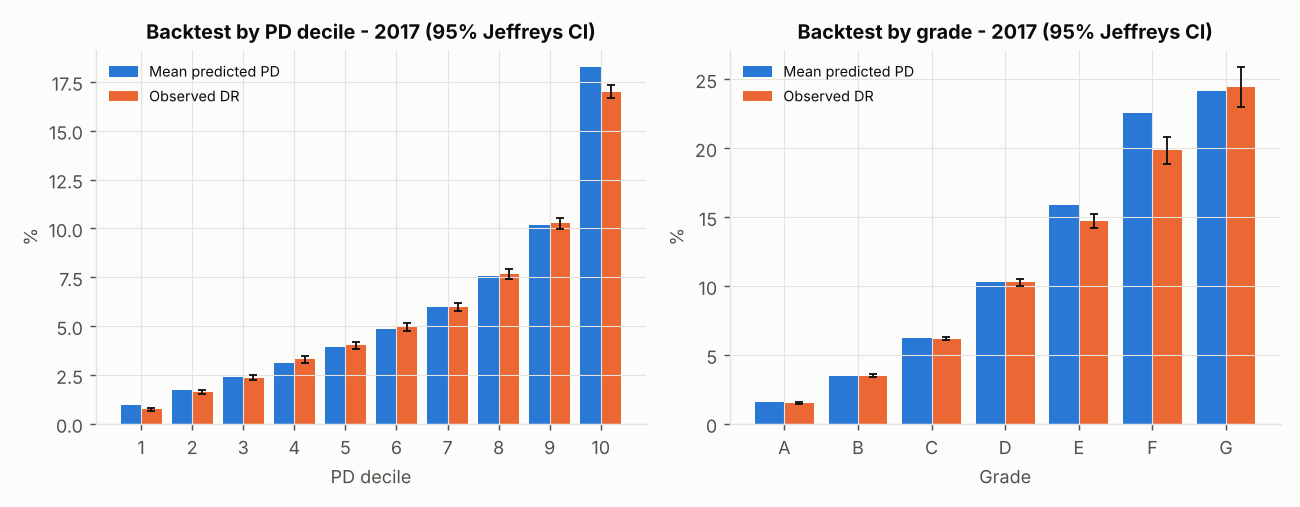
\includegraphics[width=\textwidth]{08_backtest.png}
\caption{Predicted PD vs observed default rate with 95\% Jeffreys intervals.}
\end{figure}

\textbf{Result.} Grades: 5 green, 2 conservative, no red or amber (grade D was red under Platt alone: 9.76\% vs 10.27\%). Deciles: 7 green, 2 conservative, 1 amber (decile 4: 3.13\% vs 3.30\%).

%=====================================================================
\section{Stability and vintage analysis}
%=====================================================================
\textbf{Population stability index.} With expected (development) shares $e_k$ and actual shares $a_k$ over 10 score deciles of the development sample plus a missing bin,
\begin{equation}
\mathrm{PSI}=\sum_{k}(a_k-e_k)\ln\frac{a_k}{e_k};\qquad <0.10 \text{ stable},\ 0.10\text{--}0.25 \text{ monitor},\ >0.25 \text{ significant shift}.
\end{equation}
The characteristic stability index (CSI) is the same formula applied to one feature.

\begin{figure}[H]\centering
\begin{minipage}{0.52\textwidth}\centering
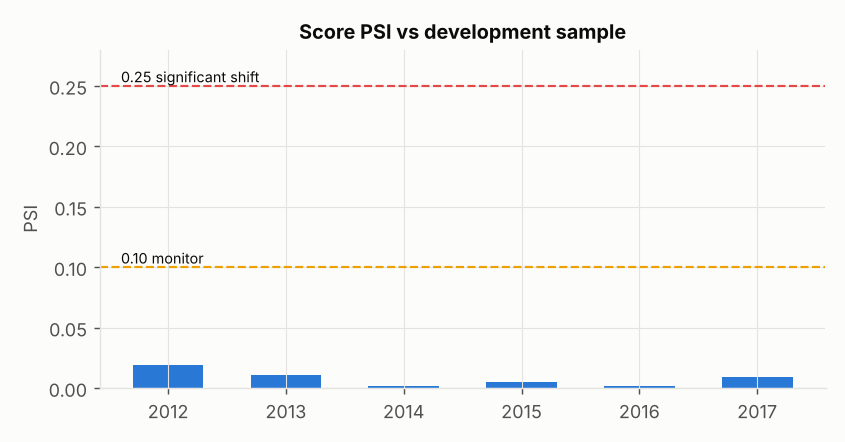
\includegraphics[width=\textwidth]{08_psi.png}
\end{minipage}\hfill
\begin{minipage}{0.4\textwidth}\centering\small
\begin{tabular}{lrl}
\toprule
Year & Score PSI & Status \\
\midrule
2012 & 0.0190 & stable \\
2013 & 0.0107 & stable \\
2014 & 0.0016 & stable \\
2015 & 0.0050 & stable \\
2016 & 0.0016 & stable \\
2017 & 0.0094 & stable \\
\bottomrule
\end{tabular}

\end{minipage}
\caption{Score PSI against the development sample: stable in every year.}
\end{figure}

\begin{table}[H]\centering\small
\caption{CSI of the top numeric features. Large values against the full development window come from the missing bin (fields structurally missing before 2012); against a fully populated 2013--2015 reference they disappear. \texttt{int\_rate} and \texttt{bc\_util} show genuine moderate drift.}
\begin{tabular}{lrrrrr}
\toprule
Feature & vs dev 2016 & vs dev 2017 & vs 2013--15: 2016 & vs 2013--15: 2017 & Dev missing \\
\midrule
sub\_grade\_n & 0.021 & 0.045 & 0.022 & 0.045 & 0.0\% \\
int\_rate & 0.091 & 0.144 & 0.091 & 0.148 & 0.0\% \\
acc\_open\_past\_24mths & 0.595 & 0.587 & 0.009 & 0.002 & 5.3\% \\
dti & 0.007 & 0.022 & 0.003 & 0.020 & 0.0\% \\
inst\_to\_inc & 0.018 & 0.053 & 0.023 & 0.062 & 0.0\% \\
revol\_to\_inc & 0.015 & 0.034 & 0.018 & 0.038 & 0.0\% \\
mo\_sin\_old\_rev\_tl\_op & 0.883 & 0.919 & 0.020 & 0.058 & 7.6\% \\
log\_inc & 0.009 & 0.018 & 0.006 & 0.016 & 0.0\% \\
bc\_util & 0.128 & 0.182 & 0.035 & 0.104 & 6.3\% \\
mo\_sin\_old\_il\_acct & 0.119 & 0.120 & 0.006 & 0.019 & 10.5\% \\
loan\_to\_inc & 0.015 & 0.044 & 0.021 & 0.052 & 0.0\% \\
mths\_since\_recent\_inq & 0.020 & 0.012 & 0.001 & 0.004 & 15.1\% \\
mths\_since\_recent\_bc & 0.102 & 0.086 & 0.006 & 0.004 & 6.2\% \\
credit\_hist\_m & 0.004 & 0.006 & 0.003 & 0.005 & 0.0\% \\
bc\_open\_to\_buy & 0.119 & 0.161 & 0.024 & 0.081 & 6.2\% \\
emp\_len & 0.011 & 0.018 & 0.011 & 0.019 & 5.1\% \\
revol\_util & 0.035 & 0.094 & 0.037 & 0.100 & 0.1\% \\
installment & 0.015 & 0.033 & 0.020 & 0.041 & 0.0\% \\
\bottomrule
\end{tabular}

\end{table}

\textbf{Vintage analysis.} For issue year $v$, the cumulative default rate at month-on-book $m$ is $\mathrm{CDR}_v(m)=\frac{1}{N_v}\sum_{i\in v}\1\{\text{status}_i\in\mathcal B,\ \tau_i\le m\}$, shown only for fully observed months.
\begin{figure}[H]\centering
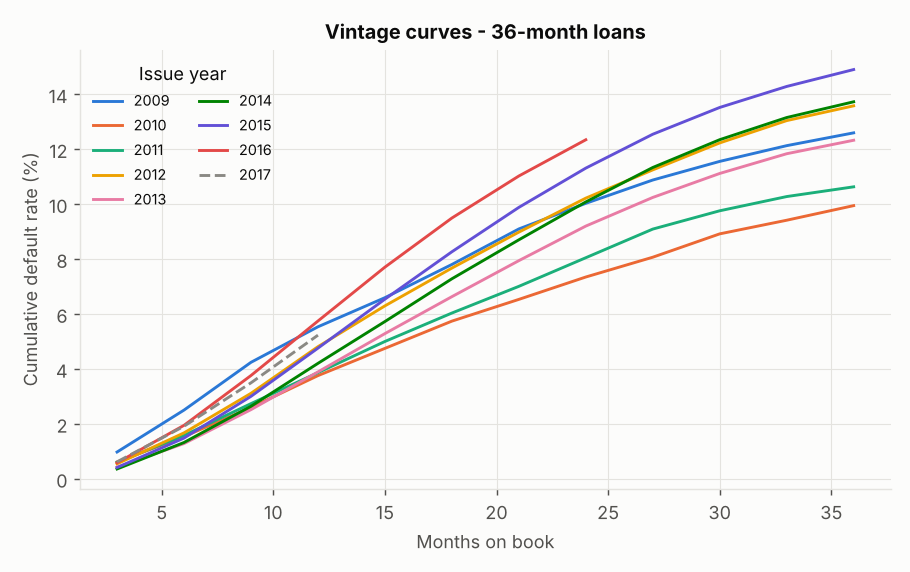
\includegraphics[width=0.75\textwidth]{03_vintage_36m.png}
\caption{Vintage curves, 36-month loans. Deterioration from 2013 to 2016: CDR at 24 months 9.2\% (2013), 10.1\% (2014), 11.3\% (2015), 12.3\% (2016).}
\end{figure}

%=====================================================================
\section{Loss given default and exposure at default}
%=====================================================================
\subsection{LGD}
For a defaulted loan,
\begin{equation}
\EAD_i=\text{Funded}_i-\text{PrincipalRepaid}_i,\qquad
\LGD_i=1-\frac{\max(\text{Recoveries}_i-\text{CollectionFee}_i,0)}{\EAD_i}\in[0,1].
\end{equation}
\textbf{Sample.} Recoveries flatten about 18 months after default, so only charge-offs at least 18 months before the snapshot are used (173{,}643 loans). Mean LGD: 0.897 (18--36 months since default) vs 0.889 (37--72 months), Welch $p\approx10^{-52}$ but only 0.9\,pp apart. OOT split by default date: train $<$ July 2015 ($n=36{,}761$), test July 2015 -- September 2017 ($n=136{,}882$).

\textbf{Fractional logit} (Papke--Wooldridge): $\E[\LGD\mid\bm x]=\Lambda(\bm x'\bm\beta)$, estimated by Bernoulli quasi-maximum likelihood $\max_{\bm\beta}\sum_i[y_i\ln\Lambda(\bm x_i'\bm\beta)+(1-y_i)\ln(1-\Lambda(\bm x_i'\bm\beta))]$ with HC1 robust standard errors (consistent for $y\in[0,1]$).

\textbf{Diebold--Mariano style test} against the mean benchmark: $d_i=(y_i-\hat y^{bench}_i)^2-(y_i-\hat y^{model}_i)^2$, $t=\bar d/(s_d/\sqrt n)$, one-sided $H_1:\E d>0$.

\begin{table}[H]\centering
\caption{LGD models, out-of-time.}
\resizebox{\textwidth}{!}{\begin{tabular}{lrrrrrrrr}
\toprule
Model & Mean obs. & Mean pred. & RMSE & MAE & $R^2_{oos}$ & Spearman & DM $t$ vs mean & $p$ (1-sided) \\
\midrule
mean & 0.8954 & 0.8954 & 0.1169 & 0.0735 & -0.0000 & -- & -- & -- \\
segment\_grade\_term & 0.8954 & 0.8952 & 0.1170 & 0.0736 & -0.0023 & 0.049 & -8.38 & 1.0000 \\
frac\_logit\_glm & 0.8954 & 0.8899 & 0.1168 & 0.0755 & 0.0015 & 0.115 & 1.62 & 0.0522 \\
lightgbm\_xentropy & 0.8954 & 0.8877 & 0.1173 & 0.0771 & -0.0072 & 0.096 & -6.58 & 1.0000 \\
\bottomrule
\end{tabular}
}
\end{table}

\textbf{Decision.} No borrower-level model beats the mean out-of-time (GLM $p=0.052$; segment and GBM are significantly \emph{worse}). LendingClub recoveries come mostly from bulk debt sales, which are not driven by borrower characteristics. Hence $\LGD=\overline{\LGD}=\mathbf{0.8954}$ (long-run, default-weighted). \textbf{Downturn LGD} $=\max_y\overline{\LGD}_y$ over default years with $\ge1{,}000$ defaults $=\mathbf{0.9363}$ (2012).

\begin{figure}[H]\centering
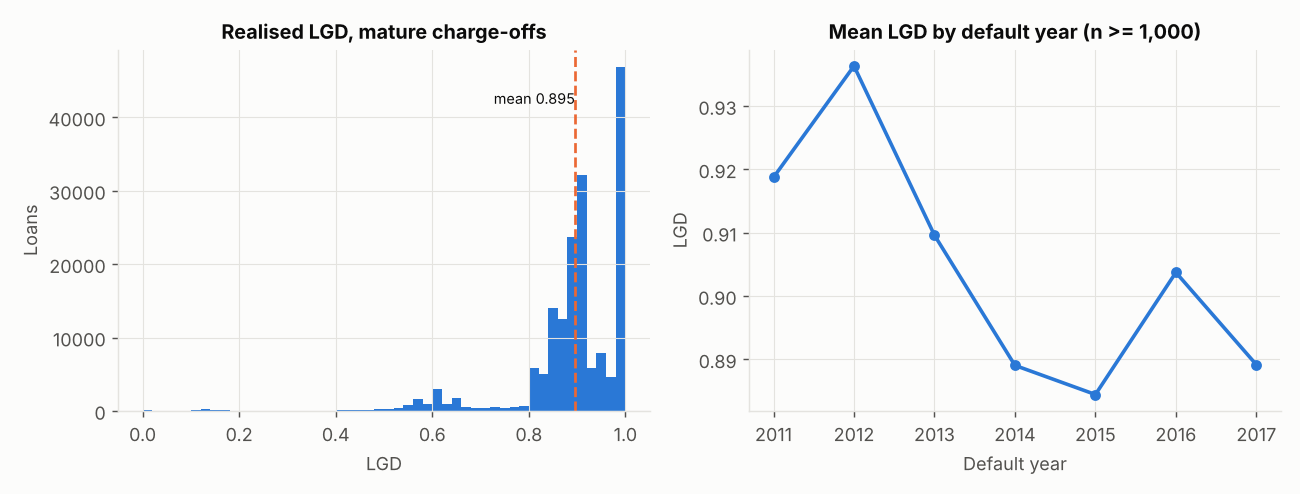
\includegraphics[width=\textwidth]{08_lgd.png}
\caption{Distribution of realised LGD and mean LGD by default year.}
\end{figure}

\subsection{EAD}
For loans defaulting within 12 months, the EAD ratio $r_i=\EAD_i/\text{Funded}_i$ (outstanding principal share at default) is modelled with a fractional logit using term, interest rate, log amount, FICO, DTI, revolving utilisation, log income, home ownership and purpose. OOT: train issue years 2007--2015, test 2016 ($n=27{,}261$).
\begin{table}[H]\centering
\caption{EAD-ratio models, out-of-time.}
\resizebox{\textwidth}{!}{\begin{tabular}{lrrrrrrrr}
\toprule
Model & Mean obs. & Mean pred. & RMSE & MAE & $R^2_{oos}$ & Spearman & DM $t$ vs mean & $p$ (1-sided) \\
\midrule
mean & 0.8731 & 0.8744 & 0.0762 & 0.0632 & -0.0003 & -- & -- & -- \\
segment\_term & 0.8731 & 0.8685 & 0.0662 & 0.0517 & 0.2447 & 0.521 & 50.14 & $<10^{-299}$ \\
frac\_logit\_glm & 0.8731 & 0.8707 & 0.0642 & 0.0497 & 0.2912 & 0.542 & 54.43 & $<10^{-299}$ \\
\bottomrule
\end{tabular}
}
\end{table}
The GLM is clearly better than the mean ($R^2_{oos}=0.29$, DM $t=54.4$). Longer terms and higher rates mean slower amortisation and therefore higher EAD.

%=====================================================================
\section{Expected credit loss}
%=====================================================================
\subsection{Formulas}
\begin{equation}
\ECL^{12m}=\sum_{i}\PD^{12m}_i\cdot\LGD\cdot\EAD^{12m}_i,\qquad \EAD^{12m}_i=\hat r_i\cdot\text{Funded}_i .
\end{equation}
\textbf{Lifetime PD.} Using the cumulative hazard $H=-\ln(1-\PD)$ and assuming a proportional hazard term structure within grade $g$ and term $t$, estimated on fully matured vintages (36m: 2012--2015, 60m: 2012--2013):
\begin{align}
k_{g,t}&=\frac{\ln(1-\mathrm{CDR}^{life}_{g,t})}{\ln(1-\mathrm{CDR}^{12m}_{g,t})},\qquad
\PD^{life}_i=1-(1-\PD^{12m}_i)^{k_{g,t}},\\
\ECL^{life}&=\sum_i\PD^{life}_i\cdot\LGD\cdot\bar r^{life}_{g,t}\,\text{Funded}_i .
\end{align}

\begin{table}[H]\centering\small
\caption{PD term structure from matured vintages.}
\begin{tabular}{lrrrrrr}
\toprule
Grade & Term & $n$ & CDR$_{12}$ & CDR$_{life}$ & $k$ & EAD ratio (life) \\
\midrule
A & 36 & 133,275 & 1.26\% & 5.45\% & 4.409 & 0.507 \\
A & 60 & 770 & 1.82\% & 8.31\% & 4.729 & 0.606 \\
B & 36 & 202,361 & 2.97\% & 11.23\% & 3.952 & 0.539 \\
B & 60 & 5,505 & 2.92\% & 15.11\% & 5.520 & 0.632 \\
C & 36 & 156,094 & 5.76\% & 18.04\% & 3.354 & 0.581 \\
C & 60 & 15,414 & 4.21\% & 21.73\% & 5.697 & 0.653 \\
D & 36 & 72,843 & 8.75\% & 23.57\% & 2.934 & 0.621 \\
D & 60 & 8,299 & 6.75\% & 27.53\% & 4.610 & 0.699 \\
E & 36 & 20,542 & 12.26\% & 28.92\% & 2.609 & 0.655 \\
E & 60 & 8,218 & 8.31\% & 32.04\% & 4.451 & 0.723 \\
F & 36 & 4,054 & 15.34\% & 33.18\% & 2.420 & 0.685 \\
F & 60 & 4,997 & 10.83\% & 36.30\% & 3.936 & 0.742 \\
G & 36 & 466 & 22.75\% & 39.91\% & 1.974 & 0.736 \\
G & 60 & 1,086 & 12.34\% & 37.94\% & 3.622 & 0.762 \\
\bottomrule
\end{tabular}

\end{table}

\begin{figure}[H]\centering
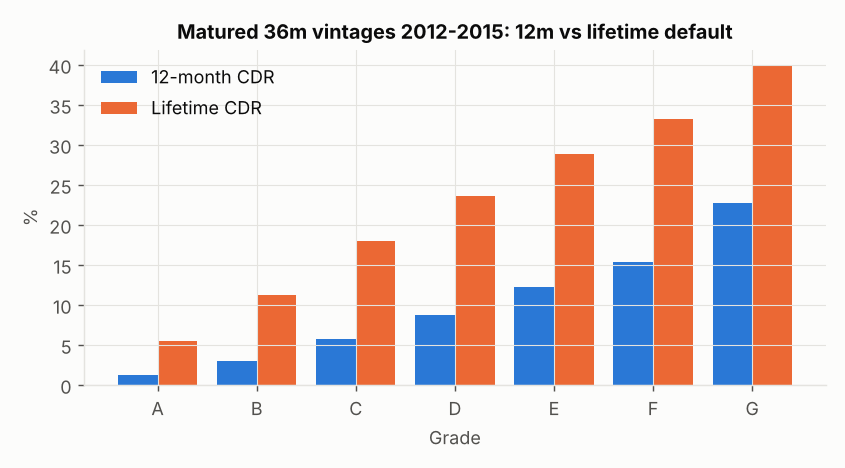
\includegraphics[width=0.68\textwidth]{08_term_structure.png}
\caption{12-month vs lifetime cumulative default rate, matured 36-month vintages.}
\end{figure}

\subsection{Results for the 2017 cohort}
\begin{table}[H]\centering
\caption{ECL by grade, 2017 cohort (443{,}579 loans, \$6{,}585.0M funded; LGD $=0.8954$).}
\resizebox{\textwidth}{!}{\begin{tabular}{lrrrrrrrrr}
\toprule
Grade & Loans & Funded \$M & PD$_{12}$ & ODR$_{12}$ & PD$_{life}$ & ECL$_{12}$ \$M & \% & ECL$_{life}$ \$M & \% \\
\midrule
A & 78,796 & 1,096.9 & 1.59\% & 1.53\% & 6.77\% & 12.4 & 1.13\% & 33.0 & 3.01\% \\
B & 133,127 & 1,839.7 & 3.50\% & 3.51\% & 13.73\% & 48.0 & 2.61\% & 130.4 & 7.09\% \\
C & 145,144 & 2,224.9 & 6.20\% & 6.19\% & 22.79\% & 105.4 & 4.74\% & 293.2 & 13.18\% \\
D & 56,646 & 891.9 & 10.27\% & 10.27\% & 30.95\% & 73.4 & 8.23\% & 170.9 & 19.16\% \\
E & 20,167 & 340.7 & 15.89\% & 14.73\% & 43.82\% & 45.1 & 13.24\% & 98.6 & 28.94\% \\
F & 6,242 & 118.6 & 22.55\% & 19.85\% & 57.52\% & 22.5 & 18.98\% & 45.8 & 38.61\% \\
G & 3,457 & 72.3 & 24.17\% & 24.41\% & 57.14\% & 14.8 & 20.42\% & 28.5 & 39.35\% \\
\textbf{Total} & 443,579 & 6,585.0 & 5.90\% & 5.80\% & 19.98\% & 321.5 & 4.88\% & 800.4 & 12.15\% \\
\bottomrule
\end{tabular}
}
\end{table}

\begin{figure}[H]\centering
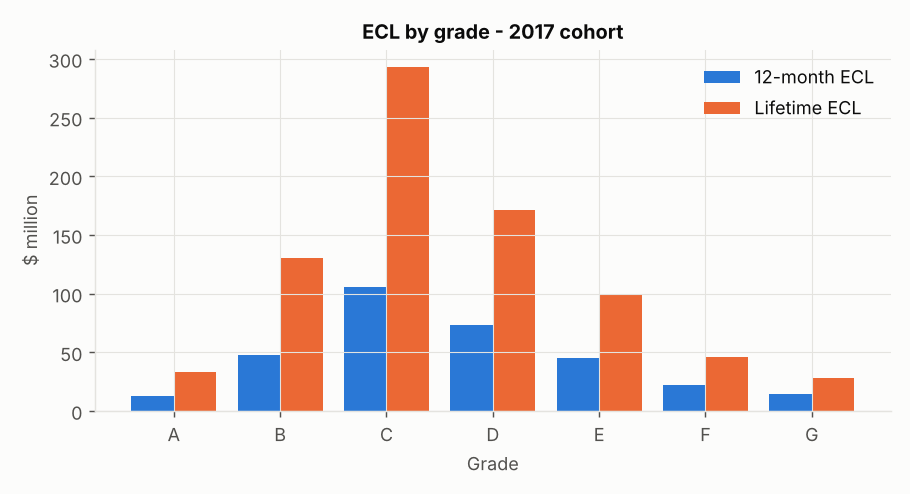
\includegraphics[width=0.68\textwidth]{08_ecl_grade.png}
\caption{12-month and lifetime ECL by grade.}
\end{figure}

\begin{keybox}[ECL results and backtest]
\begin{itemize}[leftmargin=*,itemsep=1pt]
\item 12-month EAD $=\$5{,}719.0$M; $\ECL^{12m}=\mathbf{\$321.5M}$ (4.88\% of funded).
\item $\ECL^{life}=\mathbf{\$800.4M}$ (12.15\%), mean lifetime PD 19.98\%.
\item \textbf{Backtest}: realised 12-month loss $=\sum_{i:D_i=1}\EAD_i\cdot\LGD=\mathbf{\$326.1M}$; ratio realised/predicted $=1.014$. Realised EAD of defaulters \$364.2M vs predicted $\sum\PD_i\EAD_i=\$359.1$M.
\item An independence-only test $z=(L^{real}-\ECL)/\sqrt{\sum(\LGD\,\EAD_i)^2\PD_i(1-\PD_i)}=2.08$ ($p=0.04$) ignores default correlation; under the correlated loss distribution of Section~\ref{sec:port} the realised loss is at the 59th percentile ($p=0.82$).
\end{itemize}
\end{keybox}

%=====================================================================
\section{Portfolio credit risk: one-factor Gaussian model}\label{sec:port}
%=====================================================================
\subsection{Model}
Each borrower has a latent asset value driven by one systematic factor $Z\sim N(0,1)$ and an idiosyncratic shock $\varepsilon_i\sim N(0,1)$, independent:
\begin{equation}
A_i=-\sqrt{\rho_i}\,Z+\sqrt{1-\rho_i}\,\varepsilon_i,\qquad \text{default}_i\iff A_i<\Phi^{-1}(\PD_i).
\end{equation}
($Z>0$ is a bad state.) Conditional on $Z=z$ defaults are independent with
\begin{equation}
\PD_i(z)=\Phi\!\left(\frac{\Phi^{-1}(\PD_i)+\sqrt{\rho_i}\,z}{\sqrt{1-\rho_i}}\right),\qquad \E_Z[\PD_i(Z)]=\PD_i .
\end{equation}
Portfolio loss and risk measures:
\begin{align}
L&=\sum_{i=1}^{N}\EAD_i\cdot\LGD_i\cdot\1\{\text{default}_i\},\qquad \mathrm{EL}=\E[L]=\sum_i\PD_i\,\LGD_i\,\EAD_i,\\
\VaR_q(L)&=\inf\{\ell:P(L\le\ell)\ge q\},\qquad \ES_q(L)=\E[L\mid L\ge\VaR_q(L)],\qquad \mathrm{UL}_q=\VaR_q-\mathrm{EL}.
\end{align}
\textbf{ASRF benchmark.} For a large granular portfolio, idiosyncratic risk diversifies away and
\begin{equation}
\VaR_q(L)\approx\sum_i\EAD_i\,\LGD_i\,\Phi\!\left(\frac{\Phi^{-1}(\PD_i)+\sqrt{\rho_i}\,\Phi^{-1}(q)}{\sqrt{1-\rho_i}}\right).
\end{equation}

\subsection{Asset correlation}
\textbf{Vasicek distribution.} For a large homogeneous cohort the default rate $X$ has density
\begin{equation}
f(x;p,\rho)=\sqrt{\frac{1-\rho}{\rho}}\exp\!\left(\tfrac12\big[\Phi^{-1}(x)\big]^2-\frac{1}{2\rho}\Big(\sqrt{1-\rho}\,\Phi^{-1}(x)-\Phi^{-1}(p)\Big)^2\right).
\end{equation}
\textbf{Estimation.} 36 quarterly cohorts (2009Q1--2017Q4, $n\ge500$) with observed 12-month default rate $\mathrm{DR}_t$ and mean model PD $\bar p_t$ (risk mix). A free through-the-cycle level $c$ prevents a level bias of the PDs from being read as systematic risk:
\begin{equation}
(\hat\rho,\hat c)=\arg\max_{\rho,c}\sum_{t}\ln f\big(\mathrm{DR}_t;\Lambda(\logit\bar p_t+c),\rho\big),\qquad
\hat z_t=\frac{\sqrt{1-\hat\rho}\,\Phi^{-1}(\mathrm{DR}_t)-\Phi^{-1}(p_t)}{\sqrt{\hat\rho}} .
\end{equation}
$\rho$ is profiled over $c$; the Wald SE comes from the curvature of the profile log-likelihood. Because the 12-month windows of adjacent quarters overlap, a moving-block bootstrap (block length 4, 1{,}000 replications) gives a robust CI. Without the free level, the implied $\hat z_t$ had mean $-0.75$ (biased); a unit test confirms that the free-level estimator recovers the true $\rho$ when PDs are biased.

\begin{itemize}[itemsep=1pt]
\item Model-adjusted MLE: $\hat\rho=\mathbf{0.0037}$, Wald 95\% CI $[0.0020,0.0054]$, block bootstrap $[0.0016,0.0048]$; $\hat c=-0.185$.
\item Grade-pooled unconditional MLE: $\hat\rho=0.0164$ $[0.0130,0.0207]$ (includes underwriting drift).
\item Basel IRB ``other retail'': $\rho(\PD)=0.03\,w+0.16\,(1-w)$, $w=\dfrac{1-e^{-35\PD}}{1-e^{-35}}$; 0.046 at the mean PD, portfolio mean 0.065.
\end{itemize}
\textbf{Choice.} 2009--2017 contains no recession, so the data estimate measures benign-period co-movement and is a lower bound for tail risk. The \textbf{base case uses the Basel retail $\rho(\PD_i)$ per loan}; the data estimate is a sensitivity.

\begin{table}[H]\centering\scriptsize
\caption{Quarterly cohorts used for the correlation estimate (DR and PD in \%, $\hat z_t$ implied factor).}
\begin{tabular}{lrrrr|lrrrr}
\toprule
Quarter & $n$ & DR\% & PD\% & $\hat z_t$ & Quarter & $n$ & DR\% & PD\% & $\hat z_t$ \\
\midrule
2009Q1 & 775 & 5.16 & 7.00 & -1.02 & 2013Q3 & 37,571 & 4.47 & 5.99 & -0.89 \\
2009Q2 & 965 & 5.28 & 6.40 & -0.09 & 2013Q4 & 43,869 & 4.21 & 5.82 & -1.10 \\
2009Q3 & 1,231 & 4.55 & 5.97 & -0.72 & 2014Q1 & 47,410 & 4.25 & 5.98 & -1.25 \\
2009Q4 & 1,745 & 6.53 & 6.42 & +1.63 & 2014Q2 & 55,349 & 4.59 & 6.22 & -0.98 \\
2010Q1 & 1,953 & 4.35 & 5.87 & -0.92 & 2014Q3 & 58,726 & 4.94 & 6.50 & -0.76 \\
2010Q2 & 2,776 & 5.04 & 6.03 & +0.01 & 2014Q4 & 74,144 & 5.04 & 6.47 & -0.55 \\
2010Q3 & 3,284 & 4.11 & 6.15 & -1.73 & 2015Q1 & 84,277 & 5.21 & 6.44 & -0.26 \\
2010Q4 & 3,523 & 3.89 & 5.57 & -1.36 & 2015Q2 & 95,825 & 5.38 & 6.55 & -0.14 \\
2011Q1 & 4,126 & 4.22 & 5.93 & -1.24 & 2015Q3 & 110,489 & 5.52 & 6.48 & +0.16 \\
2011Q2 & 5,102 & 4.82 & 6.12 & -0.46 & 2015Q4 & 130,504 & 5.79 & 6.30 & +0.78 \\
2011Q3 & 5,876 & 4.95 & 5.87 & +0.09 & 2016Q1 & 133,887 & 6.10 & 6.22 & +1.30 \\
2011Q4 & 6,617 & 5.24 & 6.09 & +0.25 & 2016Q2 & 97,854 & 6.27 & 6.05 & +1.76 \\
2012Q1 & 8,076 & 5.44 & 5.84 & +0.87 & 2016Q3 & 99,120 & 6.66 & 6.54 & +1.65 \\
2012Q2 & 10,447 & 5.42 & 6.56 & -0.09 & 2016Q4 & 103,546 & 6.14 & 6.31 & +1.25 \\
2012Q3 & 16,133 & 5.41 & 6.38 & +0.11 & 2017Q1 & 96,779 & 5.57 & 5.96 & +0.91 \\
2012Q4 & 18,711 & 4.96 & 5.86 & +0.11 & 2017Q2 & 105,451 & 5.82 & 5.91 & +1.33 \\
2013Q1 & 22,706 & 4.33 & 5.78 & -0.84 & 2017Q3 & 122,701 & 6.01 & 6.13 & +1.30 \\
2013Q2 & 30,668 & 4.65 & 6.14 & -0.77 & 2017Q4 & 118,648 & 5.75 & 5.61 & +1.65 \\
\bottomrule
\end{tabular}

\end{table}

\begin{figure}[H]\centering
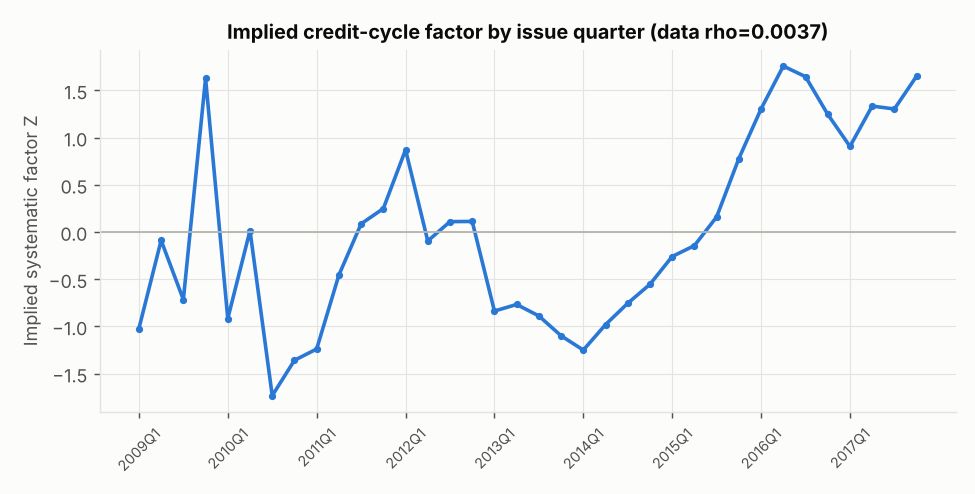
\includegraphics[width=0.78\textwidth]{06_systematic_factor.png}
\caption{Implied systematic factor by issue quarter; 2016Q2 is the worst quarter ($\hat z=1.76$).}
\end{figure}

\subsection{Monte Carlo simulation}
\begin{algorithm}[H]
\caption{Loan-level Monte Carlo (all 443{,}579 loans, $S=10{,}000$ scenarios)}
\begin{algorithmic}[1]
\State Draw $z_1,\dots,z_S\overset{iid}{\sim}N(0,1)$ \Comment{common random numbers across stress scenarios}
\For{$s=1,\dots,S$}
\State $p_{is}\gets\Phi\big((\Phi^{-1}(\PD_i)+\sqrt{\rho_i}z_s)/\sqrt{1-\rho_i}\big)$ for every loan $i$
\State Draw $u_{is}\sim U(0,1)$; $L_s\gets\sum_i \EAD_i\LGD_i\,\1\{u_{is}<p_{is}\}$
\EndFor
\State $\widehat{\mathrm{EL}}=\bar L$; $\widehat{\VaR}_q=L_{(\lceil qS\rceil)}$; $\widehat{\ES}_q=\text{mean}\{L_s:L_s\ge\widehat\VaR_q\}$
\end{algorithmic}
\end{algorithm}

\textbf{Uncertainty and validity checks.}
\begin{itemize}[itemsep=1pt]
\item \textbf{VaR CI} (distribution-free): $[L_{(j)},L_{(k)}]$ with $j=F^{-1}_{\mathrm{Bin}(S,q)}(0.025)$, $k=F^{-1}_{\mathrm{Bin}(S,q)}(0.975)$. \textbf{ES CI}: $\widehat\ES\pm1.96\,s_{tail}/\sqrt{n_{tail}}$.
\item \textbf{EL check}: $z=(\bar L-\mathrm{EL})/(s_L/\sqrt S)=-0.77$, $p=0.44$.
\item \textbf{ASRF check}: MC VaR$_{99\%}$ is $+0.96\%$ and VaR$_{99.9\%}$ $+0.69\%$ above the analytic ASRF values (\$716.8M, \$933.4M); the small excess is the granularity add-on.
\item \textbf{Original set-up} (10{,}000 loans $\times$ 2{,}000 scenarios): 99\% VaR CI width = 16.4\% of VaR, i.e.\ about $\pm8\%$ Monte Carlo error.
\end{itemize}

\begin{table}[H]\centering\small
\caption{Convergence of 99\% VaR with the number of scenarios (base case).}
\begin{tabular}{rrcr}
\toprule
Scenarios & VaR$_{99\%}$ \$M & 95\% CI \$M & CI width \\
\midrule
500 & 670.2 & [655.3, 880.8] & 33.7\% \\
1,000 & 670.0 & [652.1, 786.1] & 20.0\% \\
2,000 & 706.0 & [665.2, 750.0] & 12.0\% \\
5,000 & 726.0 & [700.6, 751.0] & 6.9\% \\
10,000 & 723.7 & [703.3, 747.3] & 6.1\% \\
\bottomrule
\end{tabular}

\end{table}

\begin{figure}[H]\centering
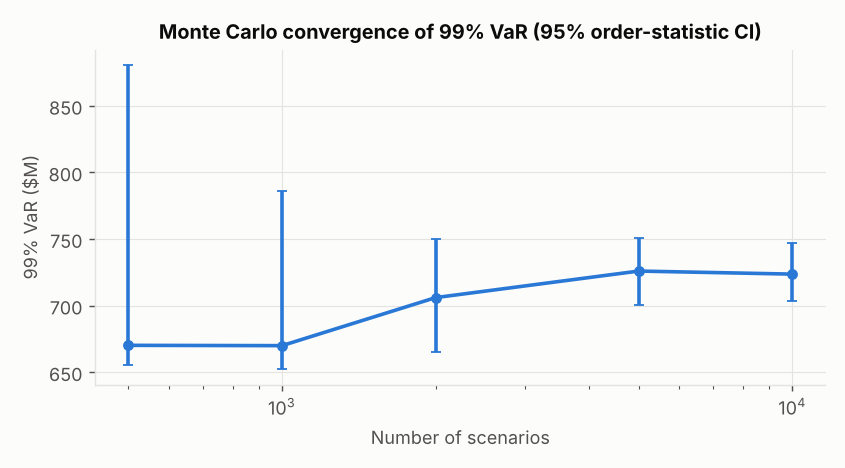
\includegraphics[width=0.62\textwidth]{08_mc_convergence.png}
\caption{Convergence of the 99\% VaR estimate.}
\end{figure}

\subsection{Base-case results}
\begin{table}[H]\centering\small
\caption{Base case: 2017 portfolio, 12-month horizon, Basel retail correlation, LGD 0.895.}
\begin{tabular}{lrr}
\toprule
Measure & Value (\$M) & 95\% CI (\$M)\\
\midrule
Expected loss (analytic / MC) & 321.5 / 320.5 & MC SE 1.3\\
Standard deviation of loss & 128.0 & \\
99\% VaR & \textbf{723.7} & [703.3, 747.3]\\
99\% ES & \textbf{820.6} & [802.6, 838.5]\\
99.9\% VaR & 939.8 & [916.0, 994.0]\\
99.9\% ES & 1{,}020.0 & [964.3, 1{,}075.6]\\
Unexpected loss (99.9\% VaR $-$ EL) & 618.3 & 9.4\% of funded\\
\bottomrule
\end{tabular}
\end{table}

\textbf{Loss backtest.} Realised 2017 12-month loss \$326.1M lies at the \textbf{58.9th percentile} of the simulated distribution: $p=2\min(\hat F(L^{real}),1-\hat F(L^{real}))=0.82$, so the model is not rejected.

\begin{figure}[H]\centering
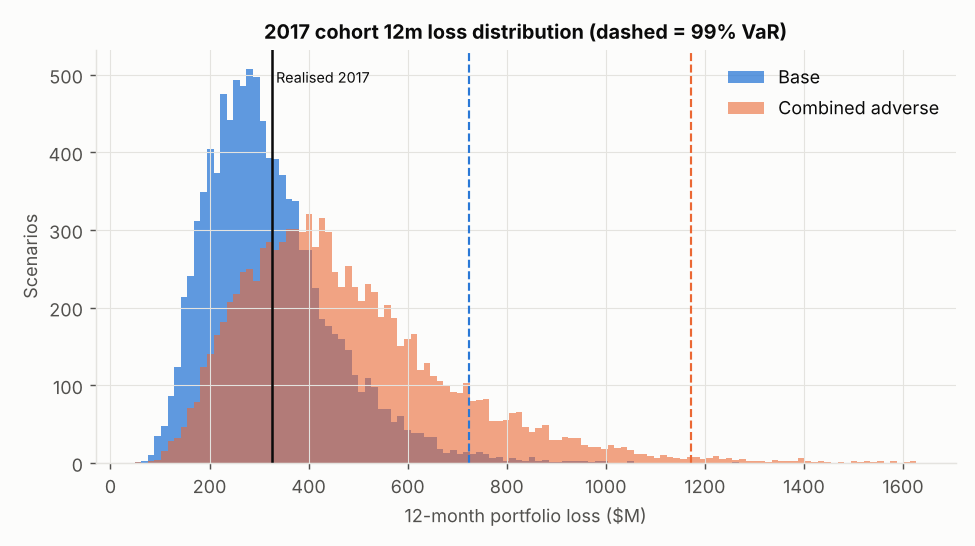
\includegraphics[width=0.85\textwidth]{06_loss_distribution.png}
\caption{Simulated 12-month loss distribution: base vs combined adverse scenario, with the realised 2017 loss.}
\end{figure}

%=====================================================================
\section{Stress testing}
%=====================================================================
All scenarios reuse the same random draws (common random numbers), so differences reflect the scenario rather than Monte Carlo noise.
\begin{itemize}[itemsep=2pt]
\item \textbf{PD odds stress}: $\PD_i'=\Lambda(\logit\PD_i+\ln m)$, $m\in\{1.5,2\}$. An odds multiplier keeps PDs in $(0,1)$ and stresses low and high PDs proportionally in odds.
\item \textbf{Historical scenario} (empirical): $m_{hist}=\max_t\dfrac{\mathrm{odds}(\mathrm{DR}_t)}{\mathrm{odds}(\Lambda(\logit\bar p_t+\hat c))}=1.249$ (2016Q2).
\item \textbf{LGD stress}: downturn LGD 0.936; LGD $+5$\,pp.
\item \textbf{Correlation stress}: $\rho_i'=\min(1.5\rho_i,0.99)$; sensitivity with the data-estimated $\rho=0.0037$.
\item \textbf{Combined adverse}: PD odds $\times1.5$ + downturn LGD + $\rho\times1.5$.
\item \textbf{Reverse stress}: find $m^*$ such that $\sum_i\Lambda(\logit\PD_i+\ln m^*)\LGD\,\EAD_i=\VaR^{base}_{99.9\%}$ (Brent's method): $m^*=\mathbf{3.74}$.
\end{itemize}

\begin{table}[H]\centering\small
\caption{Stress-test results (\$M).}
\begin{tabular}{p{7.2cm}rrrrr}
\toprule
Scenario & EL & VaR$_{99\%}$ & ES$_{99\%}$ & VaR$_{99.9\%}$ & ES$_{99.9\%}$ \\
\midrule
Base & 320.5 & 723.7 & 820.6 & 939.8 & 1,020.0 \\
PD odds x1.5 & 455.4 & 966.7 & 1,082.5 & 1,226.4 & 1,317.0 \\
PD odds x2.0 & 578.2 & 1,174.4 & 1,303.1 & 1,462.3 & 1,560.8 \\
Historical worst quarter 2016Q2 (PD odds x1.25) & 389.4 & 850.9 & 957.3 & 1,090.7 & 1,175.5 \\
Downturn LGD (0.936) & 335.2 & 756.8 & 858.1 & 982.8 & 1,066.6 \\
LGD +5pp & 338.4 & 764.1 & 866.4 & 992.3 & 1,076.9 \\
Correlation x1.5 & 320.4 & 850.8 & 988.7 & 1,160.4 & 1,276.2 \\
Data-estimated rho (0.0037, benign 2009-17) & 321.2 & 411.2 & 426.2 & 446.3 & 456.2 \\
Combined adverse: PD x1.5 + downturn LGD + rho x1.5 & 476.0 & 1,172.3 & 1,343.1 & 1,550.8 & 1,687.6 \\
\bottomrule
\end{tabular}

\end{table}

\begin{figure}[H]\centering
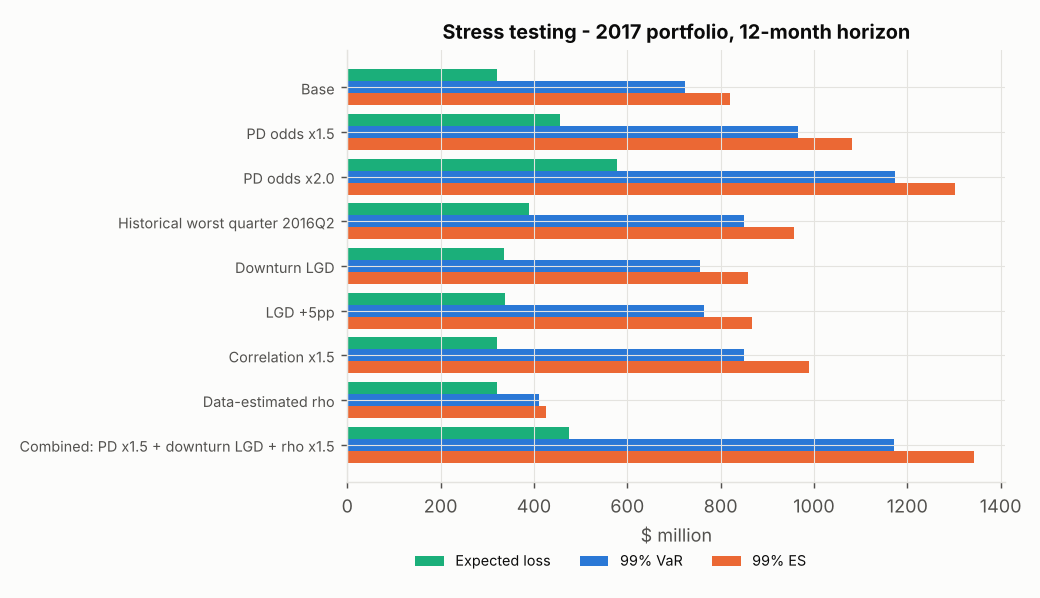
\includegraphics[width=0.85\textwidth]{08_stress.png}
\caption{Expected loss, 99\% VaR and 99\% ES by scenario.}
\end{figure}

\textbf{Interpretation.} Tail risk is driven mainly by PD level and correlation: PD odds $\times2$ raises 99\% VaR by 62\%; $\rho\times1.5$ raises it by 18\% with unchanged EL. LGD stresses move it by only about 5\% because LGD is already close to 0.9. The data-estimated correlation would cut 99\% VaR to \$411M, which is why it is not used for capital.

%=====================================================================
\section{Comparison with the original project}
%=====================================================================
\begin{table}[H]\centering\small
\caption{Original claims vs this study.}
\begin{tabular}{p{3.6cm}p{4.6cm}p{6.6cm}}
\toprule
Item & Original & This study (statistically verified)\\
\midrule
Sample / target & 1.35M terminal loans, lifetime default & 1.76M loans, 12-month default, no survivorship bias\\
2017 cohort & 169{,}321 loans, \$2.42bn & 443{,}579 loans, \$6.585bn\\
PD discrimination & LR AUC 0.700, KS 0.291, Gini 0.400 & LightGBM AUC 0.725, KS 0.325, Gini 0.450 (DeLong vs LR $p<10^{-100}$)\\
Calibration & not tested & Platt + grade; CITL $-0.02$, ECE 0.24\,pp, Jeffreys no red grade\\
LGD & assumption & empirical 0.895, downturn 0.936; OOT model tests\\
ECL & \$497.3M on \$2.42bn & 12m \$321.5M (backtest ratio 1.014); lifetime \$800.4M\\
Monte Carlo & 10k loans, 2k scenarios & 443{,}579 loans, 10k scenarios, CIs, ASRF check\\
99\% VaR / ES & \$71.4M / \$78.3M (10k-loan sample) & \$723.7M / \$820.6M (full portfolio)\\
Stress & PD odds, LGD & + historical, correlation, combined, reverse stress\\
\bottomrule
\end{tabular}
\end{table}

\section{Limitations}
\begin{itemize}[itemsep=1pt]
\item Public data only: no macro-economic covariates, no collections or recovery-process data; LGD reflects LendingClub's debt-sale recoveries.
\item The 12-month default date is reconstructed from payment information (98\% agreement with the date rule).
\item Lifetime PD extrapolates 12-month PD with hazard ratios from 2012--2015 vintages; 2017 lifetime outcomes are not yet observable.
\item The base correlation is a supervisory calibration; the observed window has no recession.
\item Hosmer--Lemeshow rejects at $N=443$k because of its high power; effect sizes are small.
\end{itemize}

\section*{Reproducibility}
Code: \texttt{src/crm} (library) and \texttt{scripts/01--09} (pipeline; \texttt{run\_all.sh}). 19 unit tests validate the statistical machinery: DeLong AUC vs scikit-learn, DeLong variance vs bootstrap, DeLong test size under $H_0$, KS vs SciPy, calibration tests on perfect and miscalibrated simulated models, PSI, Jeffreys, Holm, WOE monotonicity, Vasicek density integrating to 1, $\E[\PD(Z)]=\PD$, 95\% CI coverage of the $\rho$ MLE, free-level estimator under biased PDs, MC EL vs analytic EL, and MC VaR vs ASRF (scalar and per-loan $\rho$).

\newpage
%=====================================================================
\section{Interview questions and model answers}
%=====================================================================
\subsection*{A. Data, target and sample design}
\Q{Why did you not use only Fully Paid and Charged Off loans?}
\A For recent cohorts only loans that already ended are observed, and those are mostly early defaults and early prepayments. In 2017 only 38\% of loans had ended and their 12-month default rate was 15.1\% vs 5.8\% for all loans. That is survivorship (selection) bias. A fixed-horizon target defined for every loan removes it.

\Q{How did you define default and why a 12-month horizon?}
\A Charge-off, default or 31--120 days late with the first missed instalment within 12 months on book. 12 months is the Basel PD horizon and the IFRS~9 stage-1 horizon, and it matches the 1-year horizon of the Vasicek portfolio model.

\Q{How did you reconstruct the default date?}
\A From the last payment date when no recovery cash was received, otherwise from the number of instalments paid ($\lceil(P+Int)/A\rceil+1$). I validated the rule on 104k clean charge-offs: 98\% agreement on the 12-month flag.

\Q{What is out-of-time validation and why is it better than a random split?}
\A Train on earlier vintages and test on later ones. It mimics deployment and reveals drift in the population and in default rates; a random split would leak the 2016--2017 environment into training and overstate performance.

\Q{How did you avoid data leakage?}
\A Only origination-time fields are inputs. Payment, recovery, last-FICO, hardship and settlement fields are used only for targets, LGD and EAD. All decisions use data up to 2016; 2017 is scored once.

\subsection*{B. Feature engineering and selection}
\Q{Explain WOE and IV. What thresholds do you use?}
\A $\mathrm{WOE}_b=\ln(\%\text{bad}_b/\%\text{good}_b)$; $\mathrm{IV}=\sum(\%\text{bad}-\%\text{good})\mathrm{WOE}$. Rule of thumb: $<0.02$ useless, 0.02--0.1 weak, 0.1--0.3 medium, $>0.3$ strong (beware $>0.5$: possible leakage). I used IV $\ge0.02$.

\Q{Why monotone binning?}
\A It gives a logical, explainable relationship (risk always increases in one direction), avoids over-fitting noise in sparse bins and is expected by validators and regulators.

\Q{How did you handle multicollinearity?}
\A A $|r|>0.7$ filter in IV order before selection and a VIF $<5$ gate during selection. Example: \texttt{int\_rate} was dropped because it is almost a function of \texttt{sub\_grade}.

\Q{Why does the scorecard select only 5--12 variables?}
\A Each variable must add holdout AUC, be significant at 0.1\% and keep the right sign. LendingClub's sub-grade already prices FICO and the bureau data (FICO has Wald $p\approx0.3$ once sub-grade is in), so few variables add independent information.

\Q{How do you compare two nested logistic models?}
\A Likelihood-ratio test $2(\ell_1-\ell_0)\sim\chi^2_{\Delta k}$, plus AIC/BIC and a DeLong test on out-of-time data. v2 vs v1: $\chi^2=793$ on 7 df, $p\approx10^{-167}$, but only +0.001 AUC.

\subsection*{C. Models and discrimination}
\Q{Why is LightGBM better than logistic regression here?}
\A It captures non-linearities and interactions (e.g.\ state $\times$ grade, utilisation $\times$ income) that a WOE-additive model cannot. The gain is +0.023 AUC, highly significant by DeLong.

\Q{What is the DeLong test and why use it instead of comparing two confidence intervals?}
\A It estimates the variance and the covariance of correlated AUCs computed on the same loans; the paired test is much more powerful than checking whether separate CIs overlap.

\Q{Relationship between AUC, Gini and KS?}
\A Gini $=2\,$AUC$-1$. KS is the maximum vertical distance between the cumulative score distributions of defaulters and non-defaulters; it is a single-cut-off measure while AUC averages over all cut-offs.

\Q{Why not deploy the stacked model?}
\A It adds +0.0009 AUC: statistically significant on 443k loans but economically immaterial, while adding complexity and model-risk. Statistical significance is not the same as practical significance.

\Q{How did you tune hyper-parameters without overfitting to the test year?}
\A Random search fitted on 2007--2014 with early stopping on 2015 (time-based). 2016 was used only to choose the champion and the recalibration; 2017 was untouched.

\Q{How would you explain a LightGBM PD to a regulator?}
\A Global gain importance, SHAP values for individual decisions, monotone constraints if required, and a challenger WOE scorecard kept as the interpretable benchmark.

\subsection*{D. Calibration and backtesting}
\Q{Discrimination is good; why do you still need calibration?}
\A AUC is rank-based. ECL, capital and pricing use the PD level. Raw PDs averaged 4.8\% against an observed 5.8\% in 2017, i.e.\ ECL would be understated by about 20\%.

\Q{Platt vs isotonic vs intercept shift: how did you choose?}
\A By a rule fixed in advance on 2016: if the calibration slope differs from 1 (it was 0.92, $p\approx10^{-26}$), use Platt; then an LR test for residual grade effects ($p=10^{-19}$) justified Platt + grade.

\Q{Hosmer--Lemeshow rejects but you call the model calibrated. Why?}
\A With 443k loans HL detects basis-point deviations. I report effect sizes: mean PD 5.90\% vs 5.80\%, ECE 0.24\,pp, CITL $-0.02$ (conservative), Spiegelhalter $p=0.08$, and no red grade in the Jeffreys test.

\Q{Explain the Jeffreys test.}
\A With a Jeffreys prior Beta(1/2,1/2), the posterior of the default rate is Beta$(D+\frac12,N-D+\frac12)$. The $p$-value is the posterior probability that the true DR is below the PD; small values mean the PD is too low. It is the ECB's recommended PD backtest.

\Q{What are PSI and CSI, and what thresholds apply?}
\A $\sum(a-e)\ln(a/e)$ over bins: $<0.1$ stable, 0.1--0.25 monitor, $>0.25$ significant shift. Score PSI was 0.009 in 2017. CSI showed large values for fields missing before 2012, which I showed was a missing-bin artefact by switching to a 2013--2015 reference.

\Q{What is a vintage analysis and what did it show?}
\A Cumulative default rate by months on book for each origination cohort. Vintages deteriorated from 2013 to 2016 (24-month CDR 9.2\% $\to$ 12.3\%), consistent with the higher default rates in the OOT years.

\subsection*{E. LGD, EAD and ECL}
\Q{How did you compute LGD and why use the mean?}
\A $\LGD=1-\text{net recoveries}/\EAD$ on mature charge-offs ($\ge18$ months). A fractional logit, segment means and LightGBM did not beat the pooled mean out-of-time (Diebold--Mariano). Recoveries come from bulk debt sales, which are not borrower-driven.

\Q{What is downturn LGD and how did you estimate it?}
\A The LGD expected in an economic downturn (Basel requirement). I used the worst annual mean LGD among default years with at least 1{,}000 defaults: 0.936 (2012).

\Q{Why fractional logit for LGD and EAD?}
\A The target lies in $[0,1]$. Fractional logit keeps predictions in range and is consistent under quasi-likelihood with robust SEs (Papke--Wooldridge); OLS could predict outside $[0,1]$.

\Q{What is the difference between EL and ECL?}
\A Both are $\PD\times\LGD\times\EAD$. Basel EL uses a through-the-cycle PD and downturn LGD over one year. IFRS~9 ECL is point-in-time, forward-looking, probability-weighted, and 12-month (stage 1) or lifetime (stages 2 and 3).

\Q{How did you obtain lifetime PD?}
\A From matured vintages I estimated, per grade and term, $k=\ln(1-\mathrm{CDR}_{life})/\ln(1-\mathrm{CDR}_{12})$, a cumulative-hazard ratio, and set $\PD_{life}=1-(1-\PD_{12})^k$.

\Q{How did you backtest the ECL?}
\A Realised 12-month loss \$326.1M vs predicted \$321.5M (ratio 1.014). Placed in the correlated loss distribution, the realised loss sits at the 59th percentile ($p=0.82$). An independence-only test would wrongly reject at 5\%.

\subsection*{F. Portfolio model, VaR and ES}
\Q{Explain the Vasicek one-factor model.}
\A Each obligor's asset value is a mix of a common factor and an idiosyncratic shock; defaults are independent given the factor. The conditional PD is $\Phi((\Phi^{-1}(\PD)+\sqrt\rho z)/\sqrt{1-\rho})$. It is the basis of the Basel IRB formula (ASRF).

\Q{How did you estimate asset correlation and why not use it?}
\A MLE on 36 quarterly cohort default rates with the Vasicek density and a free level parameter, with a block-bootstrap CI: $\rho=0.0037$. The window 2009--2017 has no recession, so it understates tail dependence. I used the Basel retail correlation (mean 0.065) for the base case and the data estimate as a sensitivity.

\Q{VaR vs Expected Shortfall?}
\A VaR is a quantile and ignores losses beyond it; it is not sub-additive in general. ES is the average loss beyond VaR, is coherent, and is preferred by Basel FRTB. Base: 99\% VaR \$723.7M, 99\% ES \$820.6M.

\Q{How do you know the Monte Carlo is right?}
\A Simulated EL matches the analytic EL ($p=0.44$); simulated VaR is within 1\% of the ASRF formula; VaR converged by 5k scenarios; VaR CIs from order statistics; unit tests on simulated portfolios.

\Q{Why did you simulate the whole portfolio and not 10k loans?}
\A A sample changes the concentration (granularity) of the portfolio and the result does not scale to the real exposure; with only 2k scenarios the 99\% VaR has about $\pm8\%$ Monte Carlo error.

\Q{What is economic capital here?}
\A Unexpected loss $=$ VaR$_{99.9\%}-$EL $=\$618.3$M (9.4\% of funded).

\subsection*{G. Stress testing}
\Q{Why stress PD odds instead of multiplying PD?}
\A Multiplying PD can push it above 1 and stresses high-risk loans unrealistically; an odds multiplier keeps PDs in $(0,1)$ and is equivalent to a shift of the logit.

\Q{What drives tail risk most in your results?}
\A PD level and correlation. PD odds $\times2$: +62\% VaR; $\rho\times1.5$: +18\% VaR at the same EL; LGD stresses only about +5\% because LGD is already about 0.9.

\Q{What is a reverse stress test?}
\A Start from an outcome (loss exhausting capital) and solve for the scenario that causes it. Here PD odds must rise by $\times3.74$ before expected loss equals the base 99.9\% VaR.

\Q{How would you build a macro stress test with more data?}
\A Regress the implied systematic factor $\hat z_t$ (or default rates) on macro variables (unemployment, GDP, rates); project them under regulatory scenarios (CCAR/EBA); map to conditional PDs and recompute losses.

\subsection*{H. General and behavioural}
\Q{What was the most important finding of the project?}
\A That the original design was biased. Correcting the target changed the portfolio size from \$2.42bn to \$6.58bn and the ECL from a censored \$497M to a backtested \$321.5M (12-month).

\Q{What would you improve next?}
\A Macro-economic drivers for point-in-time PD; SHAP-based explainability and monotone constraints; a survival model for lifetime PD; a PD--LGD correlation in the portfolio model; and a monitoring pack (PSI, backtests, champion--challenger).

\Q{Statistical vs practical significance -- give an example from the project.}
\A Stacking improved AUC by 0.0009 with $p<10^{-6}$, and Hosmer--Lemeshow rejected with an ECE of only 0.24\,pp. With 443k loans almost everything is significant; decisions must also consider effect size.

\end{document}
